\documentclass[a4paper,12pt]{article}

\usepackage{jheppub}
\usepackage{taro}

\title{Mathematical Methods in Physics}

\author[a]{Taro V. Brown}

\affiliation[a]{Department of Physics, UC Davis, One Shields Avenue, Davis, CA 95616, USA }


% e-mail addresses: one for each author, in the same order as the authors
\emailAdd{taro.brown@nbi.ku.dk}
\abstract{}
\begin{document} 
\maketitle
\flushbottom
\tableofcontents
\newpage
\section{Residue Calculus}
If $f(z)$ has a pole of order $m$ at $z=a$, thrn
\begin{equation}
\Res[f(z=a)]=\frac{1}{(m-1)!}\lim_{z\to a}\dv[m-1]{}{z}[(z-a)^mf(z)]
\end{equation}
Residue theorem:
If you have some domain with poles in them, you can pinch the conbtour of integration (since it doesn't affect the end results) around these poles. $f$ is analytic in the domain and on the boundary then
\begin{equation}
\oint _C \dd z  f(z)=2\pi i \sum_{a_i\in D}\Res[f(a_i)]\end{equation}
\underline{Jordan's Lemma:} Integrals along the real line, so the contour is just the real axis, so it is open:
\begin{equation}
	\sum_{-\infty}^{\infty}f(x)\dd x= \lim_{R\to \infty }\int_{-R}^{R}f(x)\dd x
\end{equation}
to convert this to a contour integral we have to close the open segment. This can be done by making a semi circle in either the upper or the lower half-plane.
\\
Jordan's Lemma says:
Let $C_R$ be a semicircle of radius R in e.g. upper half plane (UHP) and f is analytic in UHP and decays faster than $|z|^{-1}$ for $\arg(z)\in [0,\pi]$\footnote{This argument just specifies the UHP}, then
\begin{equation}
	\int_{C_R} \dd z e^{i\alpha z}\to 0 \text{ as } R\to \infty, \text{ for } \alpha > 0
\end{equation}
This gets an exponential damping through $i\alpha z=i\alpha \Re (z)-\alpha \Im(z)$, so the integral is bounded by $1/R$ which goes to zero when we take $R\to \infty$\\
\underline{Example:}
Rational functions
\begin{equation}
\int_{-\infty}^{\infty}\frac{p(x)}{q(x)}
\end{equation}
with $p$ and $q$ begin polynomials with $q$ being one degree higher than $p$, also assume $q$ doesn't have a zero along the real line. We can the write using J's Lemma
\begin{equation}
	\int_{-\infty}^{\infty}\frac{p(x)}{q(x)}=\lim_{R\to \infty}\int_{-R}^{R}\frac{p(x)}{q(x)}\to \oint_\gamma \dd z\frac{p(z)}{q(z)}=2\pi i \sum_{a_i\in\text{UHP}}\Res[\frac{p(a_i)}{q(a_i)}]
\end{equation}
where $\gamma$ is closed contour in either UHP or LHP with LHP giving a negative sign.\\
\underline{Example I}
\begin{equation}
\begin{aligned}
\int_{0}^{\infty}\frac{x^2}{(x^2+1)(x^2+9)}&=\frac{1}{2}\int_{-\infty}^{\infty}\frac{x^2}{(x^2+1)(x^2+9)}\\
&\to \frac{1}{2}\oint_\gamma \dd z \frac{z^2}{(z^2+1)(z^2+9)}
\end{aligned}
\end{equation}
This has zeros at $z^2=1$ and $z^2=9$ so 4 simple poles at $z=\{-3i,-i,i,3i\}$. We then include the residues at these poles, so
\begin{equation}
\begin{aligned}
	&\int_{0}^{\infty}\frac{x^2}{(x^2+1)(x^2+9)}\\
	&=\frac{1}{2}2\pi i \left\{
	\Res[\frac{z^2}{(z-i)(z+i)(z+3i)(z-3i)}]_{z=i}+	\Res[\frac{z^2}{(z-i)(z+i)(z+3i)(z-3i)}]_{z=3i}
	\right\}\\
	&=\frac{1}{2}2\pi i \left\{[\frac{z^2}{(z+i)(z+3i)(z-3i)}]_{z=i}+	[\frac{z^2}{(z-i)(z+i)(z+3i)}]_{z=3i}
	\right\}\\
	&=\frac{1}{2}2\pi i \left\{\frac{i^2}{(2i)(4i)(2i)}+\frac{(3i)^2}{(3i-i)(3i+i)(3i+3i)}]
	\right\}
\end{aligned}
\end{equation}
For simple pole one can just drop the pole part and evaluate the remainder at the pole to get the residue.\\
\underline{Example II}
Sin for imaginary values is just Sinh, so $\sin(a z)\to 0$ as $Im(z)\to \pm\infty$ depending on sign of $a:\pm$. Using $\sin(az)=\Im(e^{iz})$
\begin{equation}
	\begin{aligned}
		\int_{0}^{\infty}\frac{x \sin(a x)}{(x^4+4)}&=\Im \oint_\gamma \frac{z e^{iaz}}{(x^4+4)}
	\end{aligned}
\end{equation}
This has poles at $z=\pm 1 \pm i$ so
\begin{equation}
	\begin{aligned}
		\int_{0}^{\infty}\frac{x \sin(a x)}{(x^4+4)}&=\Im \oint_\gamma \frac{z e^{iaz}}{(x^4+4)}
	\end{aligned}
\end{equation}
...\\
...\\
\underline{Example III}
Functions of trig functions
\begin{equation}
	\begin{aligned}
		\int_{0}^{2\pi} \dd \theta F(\sin \theta, \cos \theta )
	\end{aligned}
\end{equation}
with $\sin\theta = \frac{z-\frac{1}{z}}{2}$ $\cos\theta = \frac{z+\frac{1}{z}}{2}$ and $\dd \theta=\frac{\dd z}{iz}$, so
\begin{equation}
	\begin{aligned}
		I=\oint_{|z|=1} \frac{\dd z}{iz} F(\frac{z-\frac{1}{z}}{2}, \frac{z+\frac{1}{z}}{2} )
	\end{aligned}
\end{equation}
E.g.
\begin{equation}
	\begin{aligned}
		\int_{0}^{2\pi} \dd \theta \frac{1}{1+a\cos \theta}\\
		&=\frac{2}{i}\oint_{|z|=1} \frac{\dd z}{iz\left[1+a\frac{z^2+1}{2z}\right]}\\
		&=\oint_{|z|=1} \frac{\dd z}{az^2+2z+a}\\
		&=\frac{2\pi}{\sqrt{1-a^2}}
	\end{aligned}
\end{equation}
the poles are at $z=-\frac{-1\pm\sqrt{1-a^2}}{a}$\\
\underline{Principal Value Prescription (Feynman $i\epsilon$ prescription)}
If one tries to integrate a function that blows up on the real line, e.g.
\begin{equation}
\int_{-\infty}^{\infty}\frac{f(x)}{x-a}, ~~~ a\in \mathds{R}
\end{equation}
The way to integrate this is by jumping the pole on axis either below or above, so the integral is slit into
\begin{equation}
	\int_{-\infty}^{a-\epsilon}\frac{f(x)}{x-a}+\int_{a+\epsilon}^{\infty}\frac{f(x)}{x-a}+\int_\Gamma\frac{f(x)}{x-a}
\end{equation}
with $\Gamma$ the contour around the pole on the axis. Then when closing the contour using Jordan's lemma, we have to close it in the plane opposite of the the one we jumped the pole in.
The integral then gives
\begin{equation}
I = P\mp i \pi f(a)
\end{equation}
where P is the principal part (the part of the integral that ignores the divergent pole at $a$). In Feynmans language:
\begin{equation}
\frac{1}{x-a\pm i\epsilon}=P(\frac{1}{x-a})\mp i \pi\delta(x-a)
\end{equation}
\underline{Example I}\\\\
Using the Feynman Prescription
\begin{equation}
\begin{aligned}
 \int_{0}^{\infty} \dd x\frac{\sin x}{x} &=\frac{1}{2}\Im\left[ \int_{-\infty}^{\infty} \dd x\frac{e^{ix}}{x}\right]\\
 &=\frac{1}{2}\Im\left[ \int_{-\infty}^{\infty} \dd x\frac{e^{ix}}{x-i\epsilon}\right]\\
  &=\frac{1}{2}\Im\left[P \int_{-\infty}^{\infty} \dd x\frac{e^{ix}}{x-i\epsilon}+i\pi \int_{-\infty}^{\infty} \dd x e^{ix}\delta(x)\right]\\
  &=\pi/2
\end{aligned}
\end{equation}
\underline{Example II}
\begin{equation}
	\begin{aligned}
		\int_{0}^{\infty} \dd k\frac{e^{ikx}}{k^2-m^2} &=\frac{1}{2}\Im\left[ \int_{-\infty}^{\infty} \dd x\frac{e^{ix}}{x}\right]
		&=-\frac{\pi}{x}\sin(m|x|)
	\end{aligned}
\end{equation}
Often the principal is real and since we take the imaginary part, the only contribution comes from the pole 
\section{Conformal Mapping}
Very useful tool in fluid dynamics, since it is very closely tied to solving the Laplace equation in two dimensions.\\
We have seen that if $f$ is analytic then $\Re(f)$ and $\Im (f)$ are harmonic, i.e. they satisfy Laplace's equations in $d=2$ automatically from Causchy-Riemann.
\\\\
\begin{equation}
z\to f(z)
\end{equation}
we can think of this map from some domain in z-plane to $w=f(z)$. It maps points to points. So if $f$ is analytic in the first region\footnote{We only consider simply connected domains, i.e. no holes in the domains.} then it is analytic after the map.
\\\\
\underline{Riemann Mapping Theorem}
The interior of any domain $\Omega$ (with more than 1 point on $\partial\Omega$), can be conformally mapped to the unit disc $D$ with the boundary being mapped to the unit circle. The map can be made unique by choosing to map a particular point $w_0\in \Omega$ to the origin of $D$ and by orienting a particular directions from $w_0$ to the real axis in $D$.
% TODO: \usepackage{graphicx} required
\begin{figure}[H]
	\centering
	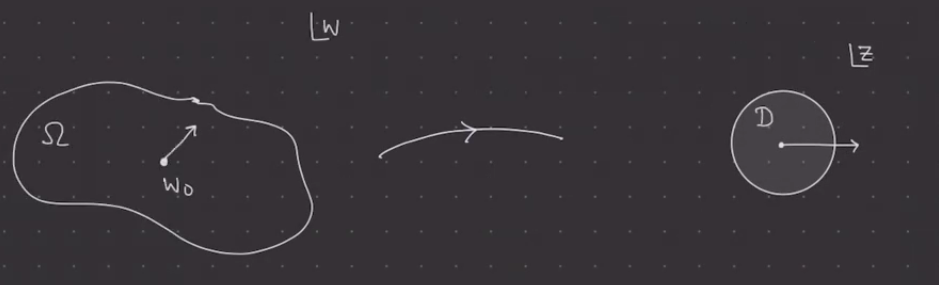
\includegraphics[width=0.7\linewidth]{3}
	\caption{}
	\label{fig:3}
\end{figure}
Let us imagine we are solving the following electrostatics problem:
\begin{equation}
\nabla^2\phi =-\delta(x)\delta(y)
\end{equation}
the potential in two dimensions behaves as
\begin{equation}
\phi\sim -\frac{1}{2\pi}\log r,~~~~~~r=\sqrt{x^2+y^2}
\end{equation}
We can map this to
\begin{equation}
	\Phi= -\frac{1}{2\pi}\log z
\end{equation}
The electrostatic potential with unit charge at $w_0$ and vanishing potential the boundary. From  $\phi$ in this domain we can construct $\Phi(w)$. Physically the situation is like punching a hole in a 2d conductor and placing a charge.
\begin{equation}
\Phi(w)=-\frac{1}{2\pi}\log (ze^{i\alpha})
\end{equation} 
is a conformal map from $w\to z$ plane which preserves the physical solution of the problem. Fixing $\alpha$, fixes a direction.\\\\
\begin{equation}
w=f(z)
\end{equation}
mapos the domain $\Omega$ to $D$. To get the inverse map $z=f^{-1}(w)$ we demand $f'(z)\neq 0$. IF
\begin{equation}
f=u+iv
\end{equation}
Then $\nabla^2u=\nabla^2 v=0$ and $u$ can be viewed as a solution to 3 dimensional Laplace equations if we have cylindrical symmetry. Let us use this to understand some problems we have already seen before.\\\\
Take $\phi=u= \Re f$ as the electrostatic potential, lines of constant $u$ gives equipotential. $v$ is field lines.\\\\
\underline{Example}
Uniform charge density wire along $z=x_3$. The equipotentials are circles and field lines go straight out.
\begin{figure}[H]
	\centering
	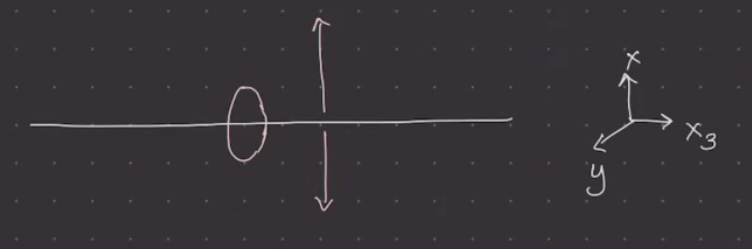
\includegraphics[width=0.7\linewidth]{4}
	\caption{}
	\label{fig:4}
\end{figure}
We have
\begin{equation}
\begin{aligned}
\Phi&=2\lambda \log z\\
\phi&=2\lambda \log r
\end{aligned}
\end{equation}
The equipotentials are $\Re[\Phi]=constant$ give circles in $x,y$ plane. Field lines come from $\Im(\phi)=2\lambda \Theta$.
\\\\
\underline{Example II}
\\\\
Two semi-infinite capacitor places at $y={\pi,-\pi}$ and hold them at constant potential $V(y=\pm \pi)=\pm \pi$. Sketching this, we now the equipotentials just go along the direction of the plates. We can use the exponential map to open it up to (almost) the whole complex plane, so taking $z\to1+z+e^z$. This maps a strip and maps it to the complex plane with two cuts. We can then solve the Laplace equation in the complex plane, i.e. we just get a linear function and the B.C.'s force the solutions to be non-zero.\\\\
The exponential map takes the complex plane and wraps it into a cylinder.
\begin{figure}[H]
	\centering
	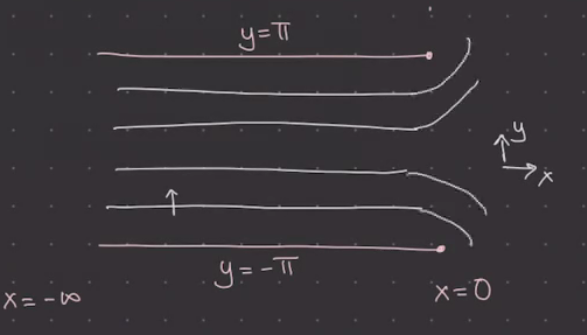
\includegraphics[width=0.7\linewidth]{5}
	\caption{}
	\label{fig:4}
\end{figure}
\begin{itemize}
\item Conformal maps are angle preserving (generally true in arbitrary dimensions)
\item In higher dimensions the full set of conformal maps is the group $SO(d,2)$ which is an extension of the Lorentz group (rotations and boost) SO($d-1,1$).
\item In 2 dimensions the conformal group is much richer: space of analytic maps. So any function $f(z)$ is a conformal transformation. This will be used later to construct interesting domain maps.
\item Subset of conformal maps: fractional linear transformations:
\begin{itemize}
	\item \begin{equation}
		w=\frac{az+b}{cz+d},~~~~~~ad-bc\neq0
	\end{equation}
	\item Translations $w=z+b$ (i.e. $c=0,d=1$)
	\item Scalings $w=\lambda z$ with $\lambda\in \mathds{R}_+$
	\item Rotations $w=e^{i\phi}z$
	\item Inversions $w=\frac{1}{z}$, analytic on $\mathds{C}/\{0\}$ maps interior of punctured disc to its exterior
 \end{itemize}
\end{itemize}
Think of $a,b,c,d$ parameterizing invertable $2\times 2$ matrices living in $GL(2,\mathds{C})$
\begin{equation}
A\begin{pmatrix}
a & b \\c& d
\end{pmatrix}
\end{equation}
If $\det A=ad-bc=1$ them we restrict to $SL(2,\mathds{C})$. \\\\
\underline{Riemann sphere}
The tranformations with $\det A=1$ transform the unit sphere onto it self. $\mathds{P}^1=\mathds{C}\cup \infty$. $S^2\subset R^3$, $\{x_1,x_2,x_3\}$. The sphere can be seen as a sterographic projection from the complex plane onto $S^2$
\begin{equation}
x_1=\frac{z+\bar z}{|z|^2+1},~~~~x_2=\frac{1}{i}\frac{z-\bar z}{|z|^2+1},~~~~x_3=\frac{|z|^2-1}{|z|^2+1}
\end{equation}
\begin{equation}
z=\frac{x_1+ix_2}{1-x_3}
\end{equation}\\\\
\subsection{How to find conformal maps}
First let us take some examples of maps:
\underline{Example I}\\\\
\begin{equation}
w=\frac{z-1}{z+1},~~~~z=\frac{w+1}{1-w}
\end{equation}
This map takes the right half of the $z$-plane to the unit disc in $w$\\\\
\underline{Example II}\\\\
\begin{equation}
\zeta= e^{i\phi}\frac{w-a}{\bar a w-1},~~~~~~|a|<1,~~~\phi\in (-\pi,\pi]
\end{equation}
This leaves the unit disc invariant.\\\\
The general way to find a conformal map is
\begin{itemize}
\item $w=f(z)$ are $\zeta=g(w)$ analytic then $\zeta= g\circ f(z)$ is a conformal map from $z\to \zeta$ planes
\end{itemize}
\underline{Example}\\\\
We want to map a strip in the z-plane to the unit disc. We know that the exponential function maps it to the right half plane
\begin{figure}[H]
	\centering
	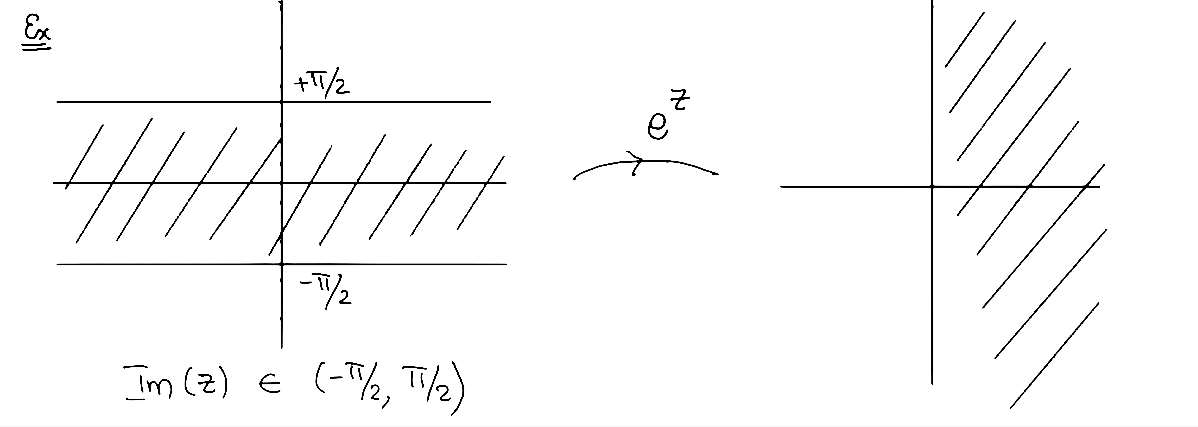
\includegraphics[width=0.7\linewidth]{7}
	\caption{}
	\label{fig:4}
\end{figure}
Now we can use the map from the half-plane to the unit sphere that we just saw and combine the two maps to get
\begin{equation}
\zeta = \frac{e^z-1}{e^z+1}
\end{equation}
\underline{Example}\\\\
To get the map from the UHP to the disc is just a combination of the right half plane map to unit disc, with a rotations:
\begin{equation}
\zeta=\frac{iz-1}{iz+1}
\end{equation}
\subsection{Applications in fluid dynamics}
We will focus on inviscid incompressible fluid and irrotational flows
\begin{equation}
\nabla\cdot \bm u=0,~~~~~~~~\nabla\times \bm u =0
\end{equation}
For 2d flow
\begin{equation}
\bm u=u_x(x,y)\hat e_x+u_y(x,y)\hat e_y
\end{equation}
The conditions on $\bm u$ imply that $u_x,u_y$ satisfy the CR relations. We can write the 2-dimensional vector field $u$ as a complex scalar $U$ as 
\begin{equation}
U(z)=u_x-iu_y
\end{equation}
Further we can write $\bm u=\nabla \phi$ and $\bm u=\nabla \times \begin{pmatrix}
1\\
1
\end{pmatrix}\chi$, with $\phi$ and $\chi$ being complex compliments and we can write
\begin{equation}
\Phi(z)=\phi(x,y)+i\chi(x,y)
\end{equation}
With
\begin{equation}
U(z)=\partial_z\Phi
\end{equation}
\underline{Example}\\\
\begin{figure}[H]
	\centering
	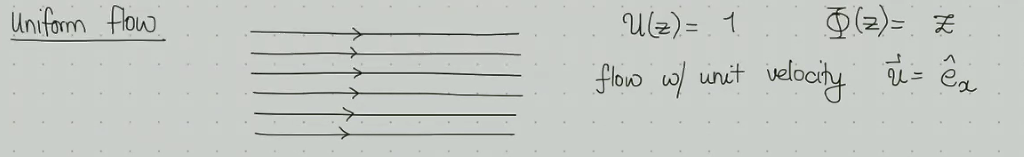
\includegraphics[width=0.8\linewidth]{8}
	\caption{}
	\label{fig:4}
\end{figure}
The streamlines are $y=c$ (constant lines) and the equipotentials are $x=c$. Now recall, analyticity of $\Phi(z)$ leads to $\grad \phi\cdot\grad \chi=0 $ since the velocity is the gradient of $\phi$ and it is tangent to $\chi=c$ then these are the level sets. If we were to add obstacles to the flow, these would be characterized by an absence of fluid flux into/out of the obstacle domain. 
\\\\
\underline{No flux condition}\\\\
$U$ is tangent to the boundary of the obstacle. $\phi$ should satisfy neumann bc at obstacle boundary
\begin{equation}
\pdv{\phi}{\bm n}
\end{equation} 
where $\bm n$ is the normal vector at the boundary.
\begin{figure}[H]
	\centering
	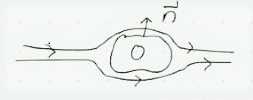
\includegraphics[width=0.6\linewidth]{9}
	\caption{}
	\label{fig:4}
\end{figure}
We will focus on flows which are asymptotically uniform, i.e. $\bm\to\hat e_x$ for $r\to \infty$ with some obstacle intermediate. Here are a few examples:
\begin{figure}[H]
	\centering
	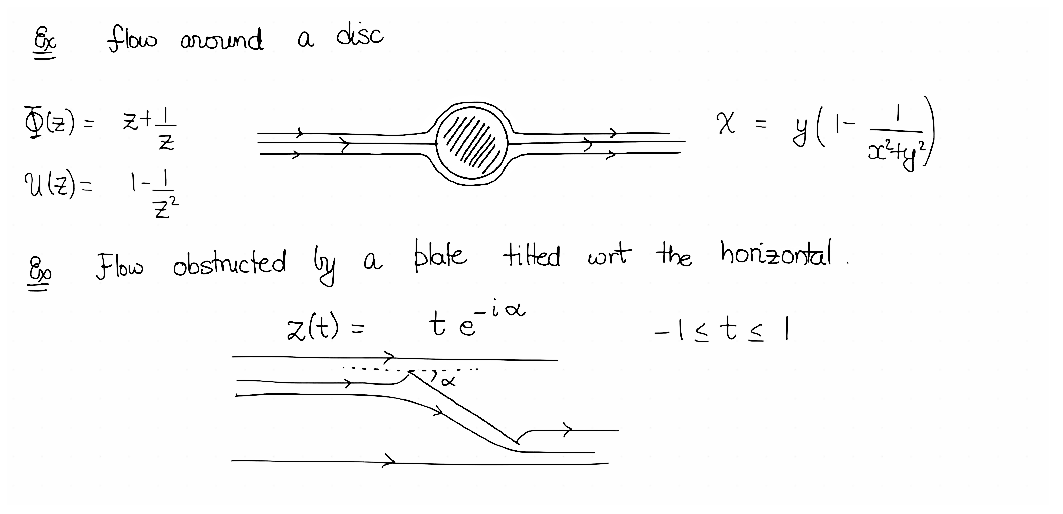
\includegraphics[width=0.9\linewidth]{10}
	\caption{}
	\label{fig:4}
\end{figure}
where $z(t)$ describes the locus of the plate
To solve the last example, we start by solving it for $\alpha=0$, so
\begin{equation}
z(t)=t,~~~~~~-1\leq t \leq 1
\end{equation}
here the solutions is clear since,
$\Phi(z)=z$. If $\alpha\neq 0$ we can solve it by rotating the plate using a conformal map. In aeronautics $\alpha$ is known as the attack angle. We will in this use the fact that rotations do not modify circular domains, which leads to the following trick:\\\\
The  Jakouwski map, mapped the unit disc to the real interval $[-1,1]$. Using this map we can go from the flow we know (at $\alpha=0$) to the unit disc, then rotate this using a rotational map, and finally map back to the $\alpha\neq 0$ solution.\\\\
The flow past a disc has then
\begin{equation}
\Phi(z)=\frac{1}{2}\left(z+z^{-1}\right)
\end{equation}
 We then rotate the disc by $\alpha$ using e.g. the map $w=e^{i\alpha}z$
 and so the jarkowski map goes to
 \begin{equation}
J(z)\to J(e^{-i\alpha})=\frac{1}{2}\left(e^{-i\alpha}w+\frac{e^{i\alpha}}{w}\right)
 \end{equation}
We then recollapse the disc by the inverse Joukoski map ($z(w)=w\pm\sqrt{w^2-1}$) and then finally rotate the solution back so that the streamlines are asymptotically horizontal, we lastly get:
\begin{equation}
\Phi(z)=e^{i\alpha}\left(z\cos \alpha -i\sin \alpha \sqrt{z^2-e^{-2i\alpha}}\right)
\end{equation}
As a pictorial example see below
\begin{figure}[H]
	\centering
	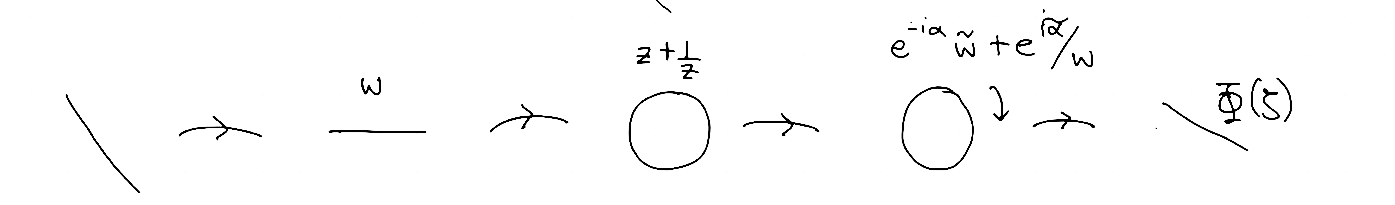
\includegraphics[width=0.9\linewidth]{11}
	\caption{}
	\label{fig:4}
\end{figure}
\section{Branch structure \& multivalued functions}
Some functions are analytic in some domain but do not have poles or essential singularities but rather something known as branchcuts. The canonical example is the function
\begin{equation}
f(z)=\log z
\end{equation}
If one writes $z=|z|e^{i\arg z}$, with $\arg z=\theta +2\pi n$,  $n\in \mathds Z$ and $\theta \in [-\pi,\pi]$. Hence we get
\begin{equation}
	f(z)=\log |z|+i\arg(z)
\end{equation}
Because $z$ and $z^{2\pi i n}$ have the same $\theta$ there is an ambiguity and hence $i\arg(z)$ is multivalued.
\begin{figure}[H]
	\centering
	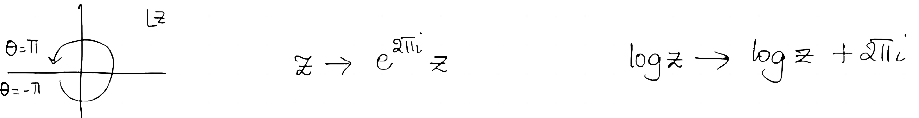
\includegraphics[width=0.9\linewidth]{12}
	\caption{}
	\label{fig:4}
\end{figure}
The origin is a branch point of $\log z$ as going around gives a discontinuous jump. Now note that
\begin{equation}
\log \frac{1}{z}=-\log z
\end{equation}
and hence there is a similar problem at $z=\infty$. This means that we can think of $\log z$ as a function in the complex plane with a line cut out of it. This line is the branchcut between the two branch points. This cut "prevents" us from going all the way around the circle, and so we never experience the discontinuity. If we instead restrict $-\pi <\theta<\pi $ on could draw this as
\begin{figure}[H]
	\centering
	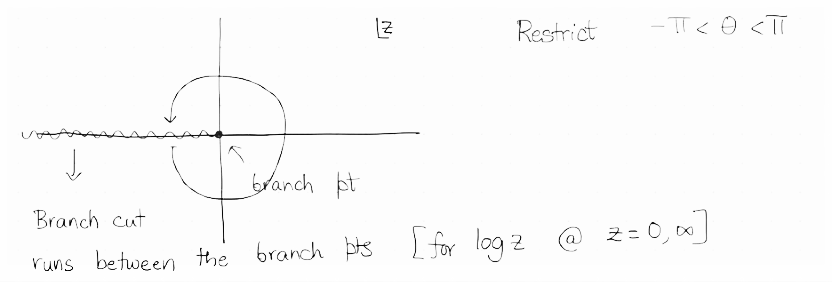
\includegraphics[width=0.9\linewidth]{13}
	\caption{}
	\label{fig:4}
\end{figure}
One can also think of this using Riemann sheets. We look at an infinite copy of complex planes and on each sheet we cut out the negative part of the real line.
\begin{figure}[H]
	\centering
	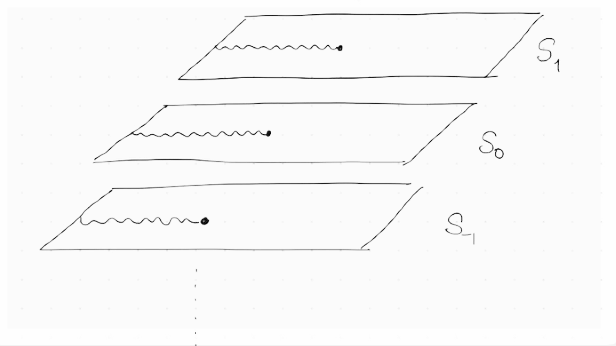
\includegraphics[width=0.9\linewidth]{14}
	\caption{}
	\label{fig:4}
\end{figure}
We then define
\begin{equation}
f_n(z)=\log |z|+i(\theta +2\pi n),~~~~\theta\in (-\pi,\pi)
\end{equation}
Slightly above and below the cut we have
\begin{equation}
\begin{aligned}
	f_n(|z|,\pi-\epsilon)&=\log |z|+i(\pi-\epsilon +2\pi n),~~~~\theta\in (-\pi,\pi)\\
		f_n(|z|,-\pi+\epsilon)&=\log |z|+i(-\pi+\epsilon +2\pi n),~~~~\theta\in (-\pi,\pi)\\
\end{aligned}
\end{equation}
across the cur we then have a discontinuiy
\begin{equation}
	\begin{aligned}
		\text{disc} f_n= \lim_{\epsilon\to 0}f_n(|z|,\pi-\epsilon)-f_n(|z|,-\pi+\epsilon)
		\end{aligned}
\end{equation}
We will then identify the "positive" side of the plane $f_{n}^+$ with $f_{n+1}^-$, so that we get the follow stairwell structure:
\begin{figure}[H]
	\centering
	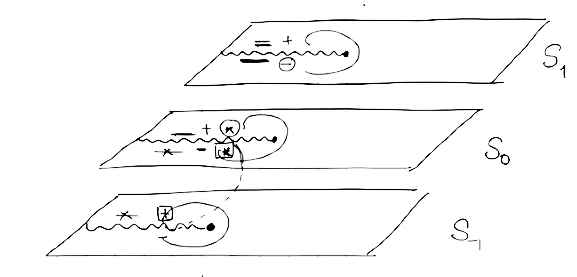
\includegraphics[width=0.9\linewidth]{15}
	\caption{}
	\label{fig:4}
\end{figure}
I.e. the $f_n$ value on the n'th sheet above the cut is equal to the $f_n$ value on (n+1)'st sheet below cut.\\\\
Since the logarithm has the property, exponentials also do. Consider for instance monomials
\begin{equation}
z^{\alpha}=e^{\alpha\log z}
\end{equation}
We then have the following cases
\begin{itemize}
\item $\alpha\in \mathds R / \mathds Q$   irrational: we have the same logarithmic cut
\item  $\alpha\in \mathds Q$ we have a finite number of sheets
\begin{itemize}
\item Example $\sqrt{z}:~~|z|^{1/2}e^{i\arg z/2}$. We can define the two phases
\begin{equation}
\sqrt{z}=\begin{cases}
&|z|^{1/2}e^{i\theta /2}\\
&|z|^{1/2}e^{i\theta z/2+i\pi}
\end{cases}
\end{equation}
The cut can be placed anywhere in the complex plane, one just has to be consistent in the convention used. 
\item Cuts can also be finite. The function $(z^2-1)^{1/2}$ e.g. has branchpoints at $z\pm 1$
\end{itemize}
\end{itemize}
Branch cuts show up a lot in 2d CFT's. Since fermions live on the double cover. Another way to put it is that since fermions behave as $\psi^\mu(x)=\psi^\mu(x+2\pi)=-\psi^\mu(x)$, which means it behaves like the squareroot function.
\subsection{Integrating functions with branch-cuts}
\underline{Example I:}
\begin{equation}
\begin{aligned}
I=\int_{0}^{\infty}\dd x \frac{x^\alpha}{1+x^2},~~~~~|\alpha|<1
\end{aligned}
\end{equation}
We convert this to a complex function
\begin{equation}
	\begin{aligned}
		I_c=\oint_{C}\dd z \frac{z^\alpha}{1+z^2},~~~~~|\alpha|<1
	\end{aligned}
\end{equation}
We first have to decide where to put the cut. Ideally we want the contour not to jump the cut. If we put the cut along the positive real axis then place our closed contour around the cut in the following way.
\begin{figure}[H]
	\centering
	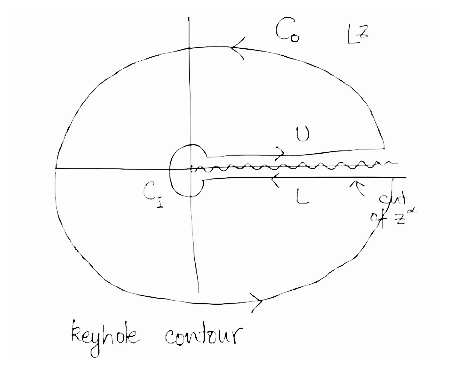
\includegraphics[width=0.7\linewidth]{16}
	\caption{}
	\label{fig:4}
\end{figure}
The contour is then
\begin{equation}
C=C_0\cup C_1\cup L\cup U
\end{equation}
On $C_0$ we have $z=Re^{i\theta}$
\begin{equation}
\begin{aligned}
	I_{C_0}=\int_{C}\dd z \frac{z^\alpha}{1+z^2}=\int_{0}^{2\pi}\dd \theta \frac{R^{1+\alpha}}{1+R^2e^{2i\theta}}e^{i(\alpha+1)\theta }
\end{aligned}
\end{equation}
This big circle doesn't contribute since
\begin{equation}
\frac{R^{\alpha+1}}{R^2}\sim \frac{1}{R^{1-\alpha}}\to 0~~~~\text{as }R\to 0 
\end{equation}
Similarly
\begin{equation}
	\begin{aligned}
		I_{C_0}=\int_{C}\dd z \frac{z^\alpha}{1+z^2}=\int_{0}^{2\pi}\dd \theta \frac{R^{1+\alpha}}{1+R^2e^{2i\theta}}e^{i(\alpha+1)\theta }
	\end{aligned}
\end{equation}
\section{Analytic continuation}
Often times one encounters a computation where there are certain limitations using real analysis, e.g. the integral has a part that is diverging. The basic idea of analytic continuation relies on the fact that complex analytic functions are very constrained, i.e. it suffices to them in a small neighborhood. This allow one to extend the definition to a larger domain while maintaining analyticity.
\\\\
As an example, let us imagine the following three domains, where we know that $f_1$ is analytic in $D_1$ and that $f_2$ is analytic in $D_2$. Further we know that $f_1=f_2$ in some common domain $D\subset D_1,D_2$. Then we conclude there must be a function which is analytic in the domain $D_1\cup D_2$.
\begin{figure}[H]
	\centering
	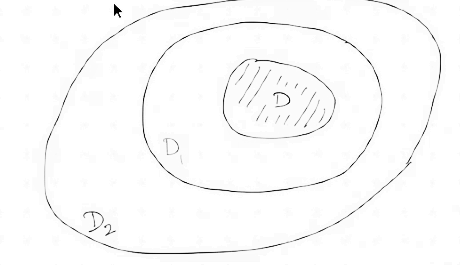
\includegraphics[width=0.5\linewidth]{17}
	\caption{}
	\label{fig:4}
\end{figure}
\underline{Example I}\\\\
Take the functions
\begin{equation}
\begin{aligned}
f_2&=\sum_0^{\infty}z^n=\frac{1}{1-z}~~~~|z|<1\\
f_2&=\sum_0^{\infty}\left(\frac{3}{5}\right)^{n+1}\left(z+\frac{2}{3}\right)^n=\frac{1}{1-z}~~~~|z+2/3|<5/3
\end{aligned}
\end{equation}
These two functions have the same representation but are valid for different domains
\begin{figure}[H]
	\centering
	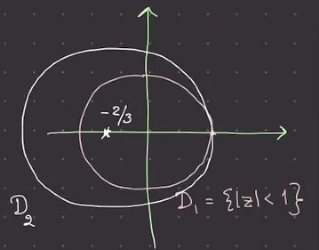
\includegraphics[width=0.5\linewidth]{18}
	\caption{}
	\label{fig:4}
\end{figure}
The function $f_2$ has been analytically continued and is valid for the much larger domain $D_2$\\\\
\underline{Example II}\\\\
We will often encounter integrals which can be analytically continued.
\begin{figure}[H]
	\centering
	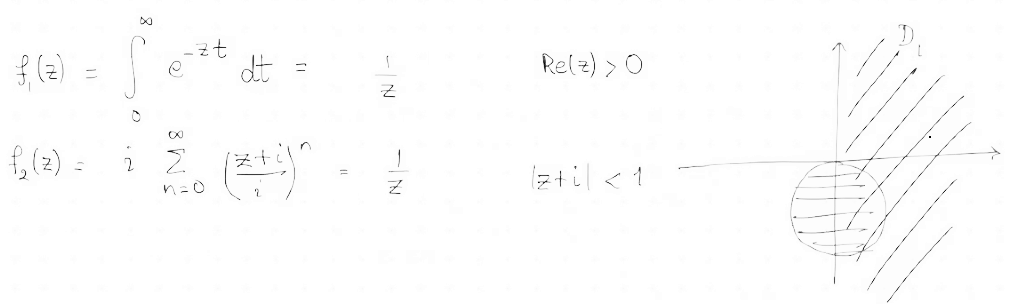
\includegraphics[width=0.8\linewidth]{19}
	\caption{}
	\label{fig:4}
\end{figure}
If you were given the first integral, one would naively think that for certain values of $z$ we would not be able to perform it, however we see that from the infinite sum one can define a version which is valid in part of the domain that was previously excluded.\\\\
\underline{Example III}\\\\
Take $\phi(x)$ to be a test function which decays rapidly enough at infinity. We then take the following integral defining an "inner product"
\begin{equation}
(x^{\alpha-1},\phi)=\int_0^\infty x^{\alpha-1}\phi(x)\dd x
\end{equation}
Notice there is an IR divergence if $\Re(\alpha)<0$. We then introduce $\epsilon$ which is known as an IR regulator and take the $\epsilon\to 0$ in the end.
\begin{equation}
\begin{aligned}
I&=\int_\epsilon^\infty x^{\alpha-1}\phi(x)\dd x\\
&=\underbrace{\frac{x^\alpha}{\alpha}\big|^{\infty}_\epsilon}_{0 \text{ for } \alpha > 0}
-\frac{1}{\alpha}\int_\epsilon^\infty x^{\alpha}\partial_x\phi(x)\dd x\\
&=-\frac{1}{\alpha}\int_\epsilon^\infty x^{\alpha}\partial_x\phi(x)\dd x
\end{aligned}
\end{equation}
This is convergent even when $-1<\Re \alpha  <0$, so this extends the definition of the original integral $I$ and together with the previous definition gives an analytic function for $\Re \alpha >-1$. There are a few caveat however, as we must assume that also the derivative of $\phi(x)$ must be sufficiently damped. The new function has pole at the origin $\alpha=0$ with residue
\begin{equation}
-\int_0^\infty \partial_x\phi(x)=\phi(0)
\end{equation}
One could use integration by parts again (and again, and again) to get
\begin{equation}
\begin{aligned}
I(\alpha)&=\frac{1}{\alpha(\alpha+1)}\int_{0}^{\infty}x^{\alpha+1}\phi''(x)\dd x
\\
&\vdots
\end{aligned}
\end{equation}
Each iteration pushed the domain one more integer into the negative $x$ axis and has poles at $\alpha=-n$ with residues \\\\
...\\\\
\underline{Gamma function}\\\\
A famous example is the function
\begin{equation}
\Gamma(z)=\int_0^{\infty}t^{z-1}e^{-t}\dd t~~~~~\Re(z)>0
\end{equation}
Repeating the same steps as before, we can write this as
\begin{equation}
	\Gamma(z)= \frac{1}{z}\int_0^{\infty}t^{z}e^{-t}\dd t=\frac{1}{z}\Gamma(z+1)
\end{equation}
Iterating this recursion one gets.
\begin{equation}
\Gamma(z)=\frac{\Gamma(z+n)}{(z+n-1)!}
\end{equation}
The residues are (at $z=-n$) given by $(-1)^n/n!$ and so we have analytically extended the gamma function to the whole complex plane with simple poles. Another definition of the gammafunction is
\begin{equation}
\frac{1}{\Gamma(z)}=\frac{1}{2\pi i}\int_C \dd \xi\, \frac{e^\xi}{z^\xi}
\end{equation}
This is defined in a very different domain. The contour $C$ is the Hankel (or hairpin) contour, see below
\begin{figure}[H]
	\centering
	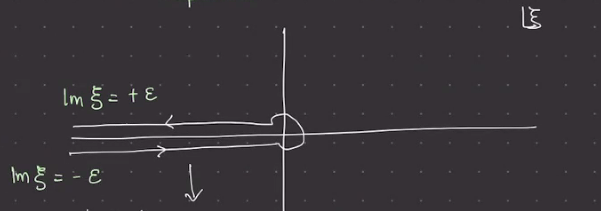
\includegraphics[width=0.7\linewidth]{20}
	\caption{}
	\label{fig:4}
\end{figure}
For positive $n$ where is no cut and the integrand can just be evaluated on the poles. By the residue theorem one finds the same as the previous definition of the gamma function.
\begin{equation}
	\frac{1}{\Gamma(z)}=\frac{1}{(n-1)!}
\end{equation}
 This is not enough to conclude the integrals describe the same function however, so let us integrate by parts
\begin{equation}
\begin{aligned}
	\frac{1}{\Gamma(z)}&=\frac{1}{2\pi i}\frac{e^{\xi}}{(z-1)\xi^{z-1}}\Big|_{-\infty-i\epsilon}^{-\infty+i\epsilon}
+
\frac{1}{z-1}\frac{1}{2\pi i}\int_C \dd \xi\, \frac{e^\xi}{z^{\xi-1}}\\
&=\frac{1}{(z-1)\Gamma(z-1)}
\end{aligned}
\end{equation}
And so we see that the recursion formula from before works for this way of expressing the gamma function as well.
\newpage
\section*{Homework 1\\\\
Taro V. Brown}\vspace*{1cm}
\section*{Problem 1}
\subsection*{Part a}
We compute
\begin{equation}
\oint_{|z|=3} \dd z\frac{4z-3}{z(z-2)}
\end{equation}
Inside the contour this has poles at $z=0$ and $z=2$ so using 
\begin{equation}
	\oint _C \dd z  f(z)=2\pi i \sum_{a_i\in D}\Res[f(a_i)]
\end{equation}
We get
\begin{equation}
\begin{aligned}
	\oint_{|z|=3} \dd z\frac{4z-3}{z(z-2)}=&2\pi i \left\{\Res[\frac{4z-3}{z(z-2)}]_{z=0}+\Res[\frac{4z-3}{z(z-2)}]_{z=2}\right\}\\
	=&2\pi i \left\{\frac{4\times 0-3}{(0-2)}+\frac{4\times 2-3}{2}\right\}\\
	=&2\pi i \left\{\frac{3}{2}+\frac{5}{2}\right\}\\	
	=&8\pi i 
\end{aligned}
\end{equation}
\subsection*{Part b}
Similarly
\begin{equation}
	\begin{aligned}
		\oint_{|z|=3} \dd z\frac{e^z}{(z-1)(z-2)}=&2\pi i \left\{\Res[\frac{e^z}{(z-1)(z-2)}]_{z=1}+\Res[\frac{e^z}{(z-1)(z-2)}]_{z=2}\right\}\\
		=&2\pi i \left\{-e+e^2\right\}\\
	\end{aligned}
\end{equation}
\section*{Problem 2}
\subsection*{Part a}
Computing
\begin{equation}
	\begin{aligned}
		\int_{0}^{\infty}\dd x\frac{2x^2-1}{x^6+1}
		=&	\frac{1}{2}\int_{-\infty}^{\infty}\dd x\frac{2x^2-1}{x^6+1}
		\\
		=&\frac{1}{2}\oint_{|z|=2} \dd z\frac{2z^2-1}{z^6+1}
	\end{aligned}
\end{equation}
$z^6+1$ has zero's within the contour at $z=\{i,(-1)^{\frac{1}{6}},(-1)^{\frac{5}{6}}\}$ and the residues can be computed by first factoring out the denominator 
\begin{equation}
(x^6+1)=(x-i)(x+i)\left(x-(-1)^{\frac{1}{6}}\right)\left(x+(-1)^{\frac{1}{6}}\right)\left(x-(-1)^{\frac{5}{6}}\right)\left(x+(-1)^{\frac{5}{6}}\right)
\end{equation}
and then applying the usual trick for first order poles. We get
\begin{equation}
\begin{aligned}
		\\
		=&\pi i
		 \left\{\Res[\frac{2z^2-1}{z^6+1}]_{z=i}+\Res[\frac{2z^2-1}{z^6+1}]_{z=(-1)^{\frac{1}{6}}}+\Res[\frac{2z^2-1}{z^6+1}]_{z=(-1)^{\frac{5}{6}}}\right\}\\
		=&\pi i \left\{\frac{i}{2}+\frac{1}{6}\left(-2i+(-1)^{\frac{1}{6}}\right)+\frac{1}{6}\left(-2i+(-1)^{\frac{5}{6}}\right)\right\}\\
		&=0
	\end{aligned}
\end{equation}

\subsection*{Part b}
For this integral we will be using $\sin n\theta =\frac{1}{2i}\left(z^n-z^{-n}\right)$, $\cos n\theta =\frac{1}{2}\left(z^n+z^{-n}\right)$ and $\dd \theta=\frac{1}{iz}\dd z$. We choose the contour $|z|=1$ since this includes all poles that show up. Computing we find
\begin{equation}
	\begin{aligned}
		\int_{0}^{\pi}\dd x\frac{\cos^2(3x)}{5-4\cos(2x)}
		=&\oint_{|z|=1}\frac{\dd z}{iz}\frac{\left(z^3+\frac{1}{z^3}\right)^2}{4 \left(1-2 \left(z^2+\frac{1}{z^2}\right)\right)}\\
		=&\oint_{|z|=1}\dd z \frac{i \left(z^6+1\right)^2}{8 z^9-4 z^7+8 z^5}\\
			=&2\pi i \left\{
			\Res[\frac{\left(z^6+1\right)^2}{8 z^9-4 z^7+8 z^5}]_{z=0}
			\right\}\\
			=&\frac{3\pi}{16}
	\end{aligned}
\end{equation}
\subsection*{Part c}
The following integral is a little tricky. First we rewrite the outer cosine at the real part of a complex function and combine the exponentials
\begin{equation}
\begin{aligned}
\int_{0}^{\pi}\dd x\, e^{\cos(x)}\cos[nx-i\sin(x)]&=\frac{1}{2}\Re\left[\int_{-\pi}^{\pi}\dd x\, e^{\cos(x)+inx-i\sin(x)}\right]\\
&=\frac{1}{2}\Re\left[\int_{-\pi}^{\pi}\dd x\, e^{inx}e^{e^{-ix}}\right]
\end{aligned}
\end{equation}
where we have used $e^{-ix}=\cos(x)-i\sin(x)$. Now
substituting $z=e^{-ix}$, which leads to $\dd z=-i e^{-ix} \dd x=-iz \dd x$
%%%%%%%%%%%%%%%%%%%%%%%%%%%%%%%%%%%%%%%%%%%%%%%%%%%%
\begin{equation}
	\begin{aligned}
\int_{0}^{\pi}\dd x\, e^{\cos(x)}\cos[nx-\sin(x)]&=\frac{1}{2}\Re\left[\int_{-\pi}^{\pi}\dd z\, \frac{e^{z}}{z^{(n+1)}}\right]\\
&=\frac{1}{2}\Re\left[\oint_{|z|=1}-i\dd z\, \frac{e^{z}}{z^{(n+1)}}\right]\\
	\end{aligned}
\end{equation}
This has an $n$'th order pole at $z=0$. We can find the residues using
\begin{equation}
	\Res[f(z=a)]=\frac{1}{(m-1)!}\lim_{z\to a}\dv[m-1]{}{z}[(z-a)^mf(z)]
\end{equation}
which in this case is particularly easy since we have an exponential function, so
\begin{equation}
	\begin{aligned}
		\int_{0}^{\pi}\dd x\, e^{\cos(x)}\cos[nx-\sin(x)]&=
		\Re\left [\pi \Res[\frac{e^{z}}{z^{(n+1)}}]_{z=0}\right]\\
		&=\frac{\pi}{n!}
	\end{aligned}
\end{equation}
\subsection*{Part d and Part e}
Lastly we have the two $\sinh$ integrals, with different contours. Let us first note that we have the Laurent series:
\begin{equation}
\frac{1}{\sinh z}=\frac{1}{z}-\frac{1}{6}z^2+\frac{7}{16}z^3+\cdots
\end{equation}
so that the combination
\begin{equation} \label{eq:sinh}
	\frac{1}{z^2\sinh z}=\frac{1}{z^3}-\frac{1}{6z}+\frac{7}{16}z+\cdots
\end{equation}
Further, we know that the zeroes of $\sinh z$ are at $n\pi i $, $n\in\mathds{Z}$ while for $z^2$ it is at $0$. This means that we for the contour $|z|=1$ only have to take the residue at $z=0$, while for $|z|=4$ also have to include the residue at $z=i\pi$. \eqref{eq:sinh} has a third order pole and a first order pole however since calculating the residue of the third order pole requires differentiating twice it's residue is just zero and we only need the contribution from the first order pole
\begin{equation}
\begin{aligned}
\oint_{|z|=1}\dd z\,\frac{1}{z^2\sinh z}  &=2\pi i \Res[\frac{1}{z^2\sinh z}]_{z=0}\\
&=2\pi i \left[-\frac{1}{6}\right]\\
&=-\frac{\pi i}{3}
\end{aligned}
\end{equation}
For the larger contour we, as mentioned, have to include the residue at $i\pi$ and $-i\pi$. The residue at this point be calculated using
\begin{equation}
\Res[\frac{p(z)}{q(z)}]_{z=a}=\lim_{z\to a}\left[\frac{p(z)}{q'(z)}\right]
\end{equation}
where $q(z)$ has a pole at $z=a$ and $p(z)$ does not. Hence taking $q(z)=\sinh(z)$ and $p(z)=z^2$  we have
\begin{equation}
\begin{aligned}
\Res[\frac{1}{z^2}\frac{1}{\sinh z}]_{z=i \pi}&=\lim_{z\to i\pi }\left[\frac{1}{z^2}\frac{1}{\cosh z}\right]\\
&=\frac{1}{\pi^2}
\end{aligned}
\end{equation}
and
\begin{equation}
	\begin{aligned}
		\Res[\frac{1}{z^2}\frac{1}{\sinh z}]_{z=-i \pi}&=\lim_{z\to -i\pi }\left[\frac{1}{z^2}\frac{1}{\cosh z}\right]\\
		&=\frac{1}{\pi^2}
	\end{aligned}
\end{equation}
So the total contour integral is
\begin{equation}
	\begin{aligned}
		\oint_{|z|=4}\dd z\,\frac{1}{z^2\sinh z}  &=2\pi i \left\{
		\Res[\frac{1}{z^2\sinh z}]_{z=0}+\Res[\frac{1}{z^2\sinh z}]_{z=i\pi}+\Res[\frac{1}{z^2\sinh z}]_{z=-i\pi}
		\right\}\\
		&=2\pi i \left[-\frac{1}{6}+\frac{1}{\pi^2}+\frac{1}{\pi^2}\right]\\
		&=2\pi i \left[-\frac{1}{6}+\frac{2}{\pi^2}\right]
	\end{aligned}
\end{equation}
\section*{Problem 3}
Using Cauchy's integral formula
\begin{equation}
	\begin{aligned}
f(a)&=\frac{1}{2\pi i}\oint_{z=|R|} \dd z\,\frac{f(z)}{z-a}
	\end{aligned}
\end{equation}
We can subtract the following term since it is zero inside this contour by Cauchy's theorem
\begin{equation}
	\begin{aligned}
		0&=\frac{1}{2\pi i}\oint_{z=|R|} \dd z\,\frac{f(z)\bar a}{ R^2-\bar az}
	\end{aligned}
\end{equation}
So we get
\begin{equation}
	\begin{aligned}
		f(a)&=\frac{1}{2\pi i}\oint_{z=|R|} \dd z\,\left[\frac{f(z)}{z-a}-\frac{f(z)\bar a}{ R^2-\bar az}\right]\\
		&=\frac{1}{2\pi i}\oint_{z=|R|} \dd z\,f(z)\frac{R^2-\bar a a}{(z-a)(R^2-\bar az)}\\
	\end{aligned}
\end{equation}
Where we have put everything on a common denominator in the last term. Expanding this denominator and writing $|a|^2=\bar a a$ we find
\begin{equation}
	\begin{aligned}
		f(a)
		&=\frac{1}{2\pi i}\oint_{z=|R|} \frac{\dd z}{z}\,f(z)\frac{R^2-|a|^2}{R^2-2\Re(a\bar z)+|a|^2}
	\end{aligned}
\end{equation}
Then letting $a=re^{i\theta}$ and integrating around the contour by setting $z=Re^{i\phi}$, $0\leq \phi \leq 2\pi$ \footnote{Note that we in the above have used $\bar z=z^{-1}$}. Further we have $\dd z=iRe^{i\phi}\dd \phi=iz\dd \phi$ and $|a|^2=r^2$, then
\begin{equation}
	\begin{aligned}
f(re^{i\theta})&=\frac{1}{2\pi i}\int_{0}^{2\pi} \dd \phi\,f(Re^{i\phi})\frac{R^2-r^2}{R^2-2Rr\cos(\theta-\phi)+r^2}
	\end{aligned}
\end{equation}
Since $f$ was assumed analytic inside the disc, this solves the Laplace equation in this region since it can be written in terms of harmonic functions through the Cauchy-Riemann conditions.
\section*{Problem 4}
\subsection*{Part a}
We have the Navier-Stokes equation:
\begin{equation}
\partial_t \bm u+\bm u\cdot  \nabla\bm u=-\nabla \left(\frac{1}{\rho} p- V\right)+\nu\nabla^2 \bm u
\end{equation}
Taking the curl on both sides we use the fact that the curl of a gradient of scalar is zero 
\begin{equation} \label{eq:ns}
	\partial_t \bm \omega+\nabla\times(\bm u \cdot \nabla\bm u)=+\nu\nabla^2 \bm w
\end{equation}
Furtherm, since $\nu=0$ in this case
\begin{equation} \label{eq:ns}
	\partial_t \bm \omega+\nabla\times(\bm u \cdot \nabla\bm u)=0
\end{equation}
Then using the fact that
\begin{equation}
\bm u \cdot \nabla\bm u=\frac{1}{2}\nabla u^2-\bm u\times (\nabla \times \bm u)=\frac{1}{2}\nabla u^2-\bm u\times \bm \omega
\end{equation}
we can rewrite
\begin{equation}
\begin{aligned}
\nabla\times(\bm u \cdot \nabla\bm u)&=\frac{1}{2}\nabla\times\nabla u^2-\nabla\times (\bm u\times \bm \omega)\\
&=\nabla\times (\bm \omega \times \bm u)\\
&=(\bm u \cdot \nabla)\bm\omega -(\bm \omega  \cdot \nabla)\bm u +\bm\omega (\nabla\cdot \bm u)+\bm u (\nabla\cdot \bm \omega )\\
&=(\bm u \cdot \nabla)\bm\omega -(\bm \omega  \cdot \nabla)\bm u
\end{aligned}
\end{equation}
where the we have used $\nabla\cdot \bm u=0$ and $\bm u(\nabla \cdot \bm \omega)=\bm u(\nabla \cdot (\nabla \times \bm u))=0$ in the third line. Inserting this back into \ref{eq:ns}:
\begin{equation} \label{eq:ns2}
	\partial_t \bm \omega+(\bm u \cdot \nabla)\bm\omega =(\bm \omega  \cdot \nabla)\bm u
\end{equation}
Or in index notation:
\begin{equation} \label{eq:ns2}
	\partial_t \omega_i+ u ^j \partial_j\omega_i = \omega^j  \partial_j u_i
\end{equation}
\subsection*{Part b}
If $\bm \omega =\nabla\times \bm u =0$, we could write
\begin{equation}
\bm u=\nabla \phi
\end{equation}
Since the equation
\begin{equation}
\nabla\times \nabla\phi =0
\end{equation}
is automatically satisfied. This is similar to the gauge potential in electrodynamics. Further from the incompressibility we know $\phi$ satisfies the Laplace equation
\begin{equation}
\nabla\cdot u=\nabla^2 \phi=0
\end{equation}
\subsection*{Part c}
First we insert $u=\nabla\phi$ into Navier-Stokes equation. Note that the following terms can be rewritten as:
\begin{equation}
\begin{aligned}
\bm u \cdot \nabla\bm u&=\frac{1}{2}\nabla u^2-\bm u\times (\nabla \times \bm u)\\
&=\frac{1}{2}\nabla u^2-\bm u\times (\nabla \times \nabla\phi)\\
&=\frac{1}{2}\nabla u^2
\end{aligned}
\end{equation}
So that we after inserting get:
\begin{equation}
	\nabla \partial_t \phi+ \frac{1}{2}\nabla \phi^2+=-\nabla \left(\frac{1}{\rho} p+ V\right)
\end{equation}
Which we can write as
\begin{equation}
	\nabla \left(\partial_t \phi+\frac{1}{2} u^2+\frac{p}{\rho} + V\right)=0
\end{equation}
This means that we can write the part in parenthesis as a constant in space but function of time $F(t)$
\begin{equation}
 \left(\partial_t \phi+\frac{1}{2} u^2+\frac{p}{\rho} + V\right)=F(t)
\end{equation}
Finally since we can just absorb the time-dependence through a shift in $\phi(t)\to\phi'$ we can write this as
\begin{equation} \label{eq:flow}
\partial_t \phi'+\frac{1}{2} u^2+\frac{p}{\rho} + V=0
\end{equation}
\subsection*{Part d}
We have already shown that since we have irrotational flow, i.e. $\nabla\times \bm u=0$ we can write the flow field as a gradient
\begin{equation}
\begin{aligned}
	u_x&=\partial_x \phi\\
	u_y&=\partial_y \phi
\end{aligned}
\end{equation}
Further, since we have an incompressible fluid, i.e. $\nabla\cdot\bm  u=0$ we can write it as a "curl" of a scalar\footnote{Since there doesn't exist such thing as a curl of scalar function, the use of curl in this case should be taken as meaning \begin{equation}
\bm u=\nabla\times \begin{pmatrix}
1\\1
\end{pmatrix}\chi
\end{equation}}
\begin{equation}
\begin{aligned}
u_x&=\partial_y \chi\\
u_y&=-\partial_x \chi
\end{aligned}
\end{equation}
since it automatically satisfies $\nabla\cdot u=0$. We see that in this case we can use either $\phi$ or $\chi$ to solve \eqref{eq:flow} and that further
\begin{equation}
	\begin{aligned}
		\partial_x \phi&=\partial_y \chi\\
		\partial_y \phi&=-\partial_x \chi
	\end{aligned}
\end{equation}
These are just the Cauchy-Riemann relations and so we we can construct an analytic function out of these, known as the stream function
\begin{equation}
\Phi=\phi+i\chi
\end{equation}
This stream-function also solves \eqref{eq:flow} since the derivatives act linearly on it as a consequence of the Cauchy-Riemann relations. This can be seen by multiplying the two sides
\begin{equation}
-\partial_x\phi\partial_x\chi=\partial_y\phi\partial_y\chi
\end{equation}
implying $(\nabla\phi)\cdot (\nabla\chi)=0$. This also implies that $\phi$ is tangent to the level sets of $\chi$. As mentioned, the terms with derivatives on $\Phi$ then become linear combinations of $\phi$ and $\chi$ and so $\Phi$ must solve the equation as well:
\begin{equation}
|\nabla \Phi|^2=(\nabla \phi+i\nabla\chi)(\nabla \phi-i\nabla\chi)=(\nabla\phi)^2+(\nabla\chi)^2
\end{equation}
\subsection*{Part e}
Here we refer to the Milne-Thomson theorem which can be used to obtain the stream-function in the case of a cylindrical obstacle through
\begin{equation}
\tilde \Phi=\Phi(z)+\bar \Phi\left(\frac{a^2}{z}\right)
\end{equation}
In this case we will assume a uniform flow with speed $u=\frac{1}{2}$ in the $x$-direction and so we have the stream-line function $\Phi(z)=\frac{1}{2}z$ and place the cylinder with $a=1$, so we get 
\begin{equation}
	\begin{aligned}
	\tilde \Phi&= \frac{1}{2}\left(z+\frac{1}{z}\right)
	\end{aligned}
\end{equation}
On the curve $|z|=1$, we have $\bar z = \frac{1}{z}$ and so the imaginary part of $\Phi$ is zero. Since $\chi=constant$ represented the constant flow streamlines, the surface of the cylinder has become a streamline and the flow doesn't penetrate this surface. This also means that the solutions holds for $|z|>1$ as prescribed in the problem.
%%%%%%%%%%%%%%%%%%%%%%%%%%%%%%%%%%%%%%%%%%%%%%%%%%
\newpage
\section*{Homework 2\\\\
	Taro V. Brown}\vspace*{1cm}
\section*{Problem 1}
\subsection*{Part a}
We will use the map provided in class
\begin{equation}
z=\frac{a}{\pi}(1+w+e^w)
\end{equation}
which maps a pair of infinite lines in the $w$ plane to a pair of semi-infinite lines in the $z$ plane. Note that the normalization in front makes sure the capacitors go from being at $a,-a$ to $-\pi,\pi$. We will analyze the lines  $w=u\pm iv$, since the equipotentials are straight lines. Inserting into the transformation:
\begin{equation}
\begin{aligned}
	z(u+iv)&=\frac{a}{\pi}(1+u+iv+e^{u+iv})\\
	&=\frac{a}{\pi}(1+u+iv+e^{u}\left[\cos v+i\sin v\right])
	\\
	&=\frac{a}{\pi}(\left[1+u+e^{u}\cos v\right]+i\left[v+e^{u}\sin v\right])
\end{aligned}
\end{equation}
From which we can identify $x$ and $y$ by setting $z=x+iy$, so
\begin{equation}
\begin{aligned}
	x&=\frac{a}{\pi}\left[1+u+e^{u}\cos v\right]\\
	y&=\frac{a}{\pi}\left[v+e^{u}\sin v\right]
\end{aligned}
\end{equation}
The potential in the infinite capacitor is $V\sim V_0v$ between the places. This potential is the imaginary part of the analytic function $\Phi(w)\sim V_0 w$. This means that varying $u$ at constant some constant $v$ will give the the equipotential lines and similarly varying $v$ at constant $u$ values give the electric field lines. We now provide a sketch of this as well as the Mathematica code written to do so. We have chosen $a=\pi$ for convenience.
\begin{lstlisting}
Potential = 
ParametricPlot[{{1 + u + Exp[u] Cos[Pi / 6], 
		Pi / 6 + Exp[u] Sin[Pi / 6]}, {1 + u + Exp[u], 
		0}, {1 + u + Exp[u] Cos[Pi / 3], 
		Pi / 3 + Exp[u] Sin[Pi / 3]}, {1 + u + Exp[u] 
		Cos[Pi / 2], 
		Pi / 2 + Exp[u] Sin[Pi / 2]}, {1 + u + Exp[u]
		Cos[2 Pi / 3], 
		2 Pi / 3 + Exp[u] Sin[2 Pi / 3]}, {1 + u + Exp[u] 
		Cos[5 Pi / 6], 
		5 Pi / 6 + Exp[u] Sin[5 Pi / 6]}, {1 + u + Exp[u] 
		Cos[8 Pi / 9], 
		8 Pi / 9 + Exp[u] Sin[8 Pi / 9]}, {1 + u + Exp[u] 
		Cos[0.97 Pi], 
		0.97 Pi + Exp[u] Sin[0.97 Pi]},
	{1 + u + Exp[u] Cos[-Pi / 6], -Pi / 6 + Exp[u] 
		Sin[-Pi / 6]}, {1 +
		u + Exp[u], 
		0}, {1 + u + Exp[u] Cos[-Pi / 3], -Pi / 3 + 
		Exp[u] Sin[-Pi / 3]}, {1 + u + Exp[u] 
		Cos[-Pi / 2], -Pi / 2 + 
		Exp[u] Sin[-Pi / 2]}, {1 + u + 
		Exp[u] Cos[-2 Pi / 3], -2 Pi / 3 + Exp[u] 
		Sin[-2 Pi / 3]}, {1 + 
		u + Exp[u] Cos[-5 Pi / 6], -5 Pi / 6 + 
		Exp[u] Sin[-5 Pi / 6]}, {1 + u + 
		Exp[u] Cos[-8 Pi / 9], -8 Pi / 9 + Exp[u] 
		Sin[-8 Pi / 9]}, {1 + 
		u + Exp[u] Cos[-0.97 Pi], -0.97 Pi + 
		Exp[u] Sin[-0.97 Pi]}}, {u, -9, 2.43}, 
PlotStyle -> {{Gray, Thick}, {Gray, Thick}}];
Plates = ParametricPlot[{{1 + u + Exp[u] Cos[Pi], 
		Pi + Exp[u] Sin[Pi]}, {1 + u + Exp[u] 
		Cos[-Pi], -Pi + 
		Exp[u] Sin[-Pi]}}, {u, -9, 2.43}, 
PlotStyle -> {{Blue, Thick}, {Blue, Thick}}];
Electric = 
ParametricPlot[{{1 + -8. + Exp[-8] Cos[v], 
		v + Exp[-8] Sin[v]}, {1 + -6. + Exp[-6] Cos[v], 
		v + Exp[-6] Sin[v]}, {1 + -4 + Exp[-4] Cos[v], 
		v + Exp[-4] Sin[v]}, {1 + -2 + Exp[-2] Cos[v], 
		v + Exp[-2] Sin[v]}, {1 + -1 + Exp[-1] Cos[v], 
		v + Exp[-1] Sin[v]}, {1 + 0 + Exp[0] Cos[v], 
		v + Exp[0] Sin[v]}, {1 + 1 + Exp[1] Cos[v], 
		v + Exp[1] Sin[v]}, {1 + 2 + Exp[2] Cos[v], 
		v + Exp[2] Sin[v]}, {1 + 1.5 + Exp[1.5] Cos[v], 
		v + Exp[1.5] Sin[v]}}, {v, -\[Pi], Pi}, 
PlotStyle -> {{Red, Dashed}, {Red, Dashed}}];
Show[Electric, Plates, Potential]
\end{lstlisting}
Which results in the following figure
\begin{figure}[H]
	\centering
	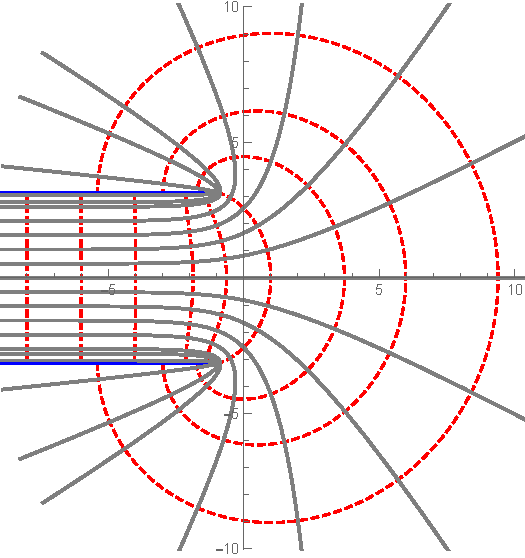
\includegraphics[width=0.7\linewidth]{hw2.pdf}
	\caption{Plot of equipotential lines (grey) and field lines (red, dashed)}
	\label{fig:4}
\end{figure}
%%%%%%%%%%%%%%%%%%%%%%%%%%%%%%%%%%%%%%%%%%%%%%%%%%
%%%%%%%%%%%%%%%%%%%%%%%%%%%%%%%%%%%%%%%%%%%%%%%%%%
%%%%%%%%%%%%%%%%%%%%%%%%%%%%%%%%%%%%%%%%%%%%%%%%%%
\subsection*{Part b}
We will here use the following map, obtained from the conformal dictionary
\begin{equation}
w=\frac{2}{\pi}\asin(z)
\end{equation}
This maps two lines to two parallel plates. The inverse, which is the one we are interested in, is
\begin{equation}
	z=\sin(\frac{2}{\pi}w)
\end{equation}
First we write it in terms of its real and complex parts using a trig identity
\begin{equation}
\begin{aligned}
	x+iy=z=\sin((u+iv)\frac{2}{\pi})=\sin\frac{\pi}{2}u\cosh\frac{\pi}{2}v+i\cos\frac{\pi}{2}u\sinh\frac{\pi}{2}v
\end{aligned}
\end{equation}
Then to find equipotentials we first identity
\begin{equation}
\begin{aligned}
x&=\sin\frac{\pi}{2}u\cosh\frac{\pi}{2}v\\
y&=\cos\frac{\pi}{2}u\sinh\frac{\pi}{2}v
\end{aligned}
\end{equation}
Then taking $u=constant$ we get
\begin{equation}
	\begin{aligned}
		\left(\frac{x}{\sin\frac{\pi}{2}u}\right)^2-\left(\frac{y}{\cos\frac{\pi}{2}u}\right)^2=\cosh^2\frac{\pi v}{2}-\sinh^2\frac{\pi v}{2}=1
	\end{aligned}
\end{equation}
or a hyperbola. Smiliar holding $v$ constant to find the field lines, we get elipses
\begin{equation}
	\begin{aligned}
		\left(\frac{x}{\cosh\frac{\pi}{2}v}\right)^2+\left(\frac{y}{\sinh\frac{\pi}{2}v}\right)^2=\cos^2\frac{\pi u}{2}+\sin^2\frac{\pi u}{2}=1
	\end{aligned}
\end{equation}
Both hyperboles and elipses are conic sections. Sketching these for different values of $u$ and $v$ we get, using the following mathematica code
\begin{lstlisting}
ContourPlot[{x^2/Sin[1]^2 - y^2/Cos[1]^2 == 1, 
	x^2/Sin[2]^2 - y^2/Cos[2]^2 == 1, 
	x^2/Sin[2.5]^2 - y^2/Cos[2.5]^2 == 1, 
	x^2/Sin[3]^2 - y^2/Cos[3]^2 == 1, 
	x^2/Cosh[1]^2 + y^2/Sinh[1]^2 == 1, 
	x^2/Cosh[2]^2 + y^2/Sinh[2]^2 == 1, 
	x^2/Cosh[2.5]^2 + y^2/Sinh[2.5]^2 == 1, 
	x^2/Cosh[3]^2 + y^2/Sinh[3]^2 == 1},
 	{x, -6.5, 6.5}, {y, -6.5, 6.5}]
\end{lstlisting}
\begin{figure}[H]
	\centering
	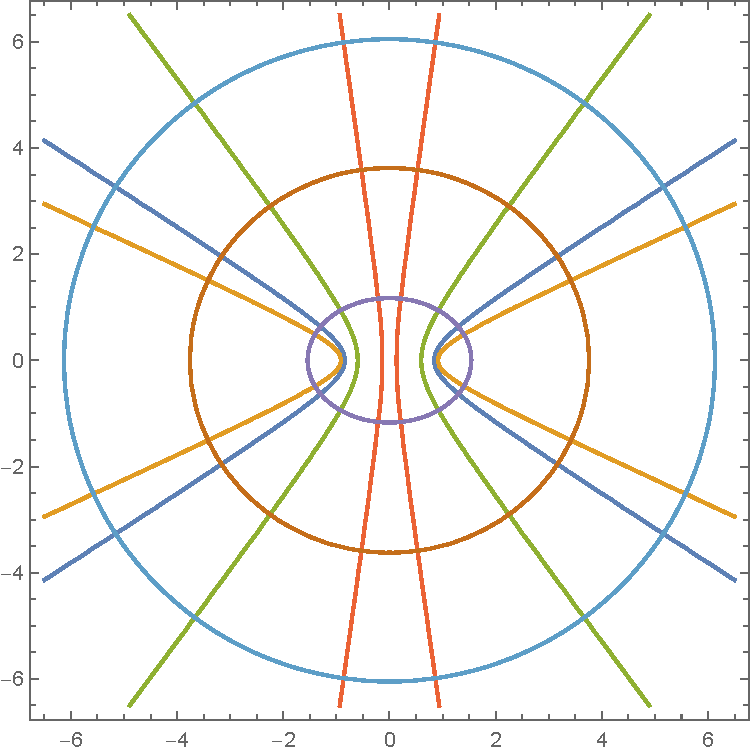
\includegraphics[width=0.7\linewidth]{contour.pdf}
	\caption{Plot of equipotential lines (parabolas) and field lines (elipses)}
	\label{fig:4}
\end{figure}
\section*{Problem 2}
The transformation that takes the unit disc to the unit disc is the linear fractional transformation
\begin{equation}
f(z)= e^{i\phi}\frac{z-\alpha}{\bar \alpha z-1},~~~~~~|\alpha|<1,~~~~~-\pi<\phi < \pi
\end{equation}
The rotation part $e^{i\phi}$ obviously just maps points in the disc to other points in the disc, while the linear fraction part moves the origin from $z=0$ to $f=\alpha$. We can show that this maps to the unit disc if $|f(z)|<1$ so that every point in the domain lies within the disc. First we note that
\begin{equation}
\begin{aligned}
|z-a|^2&=(z-a)(\bar z-\bar a)=|z|^2+|\alpha|^2-\alpha \bar z-\bar \alpha z\\
|\bar \alpha z-1|^2&=(\bar \alpha z-1)( \alpha \bar z-1)=|z|^2|\alpha|^2-\alpha \bar z-\bar \alpha z+1
\end{aligned}
\end{equation}
If we take the difference of the two we find
\begin{equation}
\begin{aligned}
|z-a|^2-|\bar \alpha z-1|^2&=|z|^2+|\alpha|^2-\alpha \bar z-\bar \alpha z-|z|^2|\alpha|^2+\alpha \bar z+\bar \alpha z-1\\
&=|z|^2+|\alpha|^2-|z|^2|\alpha|^2-1\\
&<0
\end{aligned}
\end{equation}
where the last inequality only holds since we started within the disc, $|z|<1$, and since we assumed $|\alpha|<1$. This implies that $|z-a|<|\bar \alpha z-1|$ and hence that 
\begin{equation}
\begin{aligned}
|f(z)|=\frac{|z-\alpha|}{|\bar \alpha z-1|}<1
\end{aligned}
\end{equation}
which means that every point in the new domain, lies within the unit circle.  
\section*{Problem 3}
\subsection*{Part a}
Here we will use the composition law
\begin{itemize}
	\item If $w=f(z)$ and $\zeta=g(w)$ are analytic then $\zeta= g\circ f(z)$ is a conformal map from $z\to \zeta$ planes
\end{itemize}
First we will use the following map presented in class, namely
\begin{equation}
w=\frac{z+1}{z-1}
\end{equation}
which maps the half disc $z\in D_+$ to the upper right quadrant (URQ) $w\in 0<\arg w <\frac{1}{2}\pi$. The map that takes the URQ to the unit disc is found in the conformal dictionary
\begin{equation}
 \zeta(w)=\frac{iw^2+1}{iw^2-1}
\end{equation}
Taking the composition we find
\begin{equation}
\begin{aligned}
\zeta(w=\frac{z+1}{z-1})&=\frac{i\left(\frac{z+1}{z-1}\right)^2+1}{i\left(\frac{z+1}{z-1}\right)^2-1}\\
&=\frac{-i\left(1+2iz+z^2\right)}{1-2iz+z^2}
\end{aligned}
\end{equation}
The factor $-i$ in front is the same as rotating the disc, which also leaves it invariant so a valid solution is also
\begin{equation}
	\begin{aligned}
		\zeta(z)
		&=\frac{\left(1+2iz+z^2\right)}{1-2iz+z^2}
	\end{aligned}
\end{equation}
Note that this can also be simplified to
\begin{equation}
	\begin{aligned}
		\zeta(z)
		&=1+\frac{4iz}{1-2iz+z^2}
	\end{aligned}
\end{equation}
though the fractional form might be nicer to use. One can further note that this map is not unique and by acting with the transformation found in the previous problem the disc would still be invariant and hence one could use the composition with this, to map the half disc at the origin to the unit disc centered around a different origin:
\begin{equation}
	\begin{aligned}
		\zeta 
		&=e^{i\phi}\frac{\left(1+\frac{4iz}{1-2iz+z^2}\right)-\alpha}{\bar \alpha \left(1+\frac{4iz}{1-2iz+z^2}\right)-1}\\
		&=e^{i\phi}\frac{\left(1+2iz+z^2\right)-\alpha(1-2iz+z^2)}{-1+\bar a+2i(1+\bar a)z+(-1+\bar a)z^2}
		\\
		&=e^{i\phi}\frac{\left(1+2iz+z^2\right)-\alpha(1-2iz+z^2)}{\alpha(1+2iz+z^2)-\left(1-2iz+z^2\right)},~~~~~~|\alpha|<1,~~~~~-\pi<\phi < \pi
	\end{aligned}
\end{equation}
\subsection*{Part b}
We will assume the radius of the outer circle to be 1 and inner circle to have the origin at $z=c$ with radius $c$. Basically we are looking for the following map
\begin{figure}[H]
	\centering
	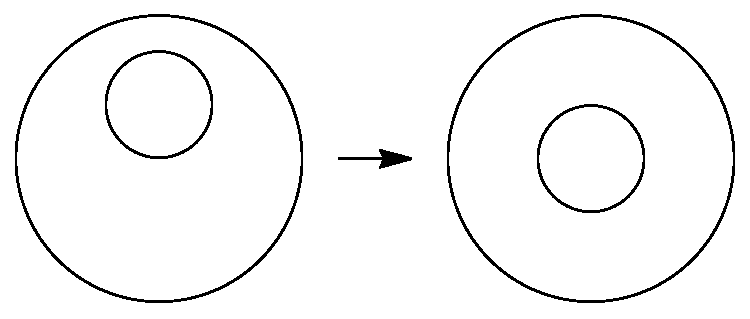
\includegraphics[width=0.7\linewidth]{map.pdf}
	\caption{Non-concentric circles to annulus}
	\label{fig:4}
\end{figure}
Using the fractional part of the transformation from problem 2, we have a map that takes circles at origin and map them to circles centered around some other point. This implies that we can use that map here and we just need to find a value of $\alpha$ which takes the inner circle with origin at $z=c$ and radius $c$ to a circle with origin at $z=0$ and radius $r$. We will assume $\alpha\in \mathds R$, so $\bar \alpha=\alpha$. Mapping the edges of the inner circle to $-r$ and $r$ we find:
\begin{equation}
\begin{aligned}
-r&=f(z=0)=\frac{0-\alpha}{\alpha\times 0-1}=\alpha
\\
r&=f(z=2c)=\frac{2c-\alpha}{2\alpha c-1}\\
\Rightarrow~~~~&2c-\alpha=-\alpha(2\alpha c-1)\\
\Rightarrow~~~~&2\alpha^2c-2\alpha+2c=0\\
\Rightarrow~~~~&\alpha^2c-\alpha+c=0\\
\Rightarrow~~~~&\alpha_\pm =\frac{1\pm\sqrt{1-4c^2}}{2c}\\
\end{aligned}
\end{equation}
The problem states that $0<c<1/2$ and since $|\alpha|<1$ the only valid solution is $\alpha_-$. Inserting this into the map, we find
\begin{equation}
\begin{aligned}
	f(z)&= \frac{z-\frac{1-\sqrt{1-4c^2}}{2c}}{\frac{1-\sqrt{1-4c^2}}{2c} z-1}\\
	&=\frac{1-\sqrt{1-4c^2}-2cz}{2c+(\sqrt{1-4c^2}-1)z},~~~~~~c<1/2
\end{aligned}
\end{equation}
\section*{Problem 4}
\subsection*{Part a}
In this problem we will be using the map from the previous problem. On could do the problem for a general $c$, but we note that (requiring, $c<1/2$) the following values of $c$ simplify the transformation
\begin{lstlisting}
In[238]:= Simplify[
Table[-((-1 + Sqrt[1 - 4 b^2] + 2 b z)/(
2 b + (-1 + Sqrt[1 - 4 b^2]) z)), {b, {1/3, 1/4, 1/5, 2/5}}]]

Out[238]= {-((-3 + Sqrt[5] + 2 z)/(
	2 + (-3 + Sqrt[5]) z)), -((-2 + Sqrt[3] + z)/(
	1 + (-2 + Sqrt[3]) z)), -((-5 + Sqrt[21] + 2 z)/(
	2 + (-5 + Sqrt[21]) z)), (-1 + 2 z)/(-2 + z)}
\end{lstlisting}
The simplest transformation happens at $c=\frac{2}{5}$ meaning the center of the small circle is at $z=\frac{2}{5}$ and the radius is $r=\frac{2}{5}$. In this case we get the simple map
\begin{equation}
	\begin{aligned}
		f(z)
		&=\frac{2z-1}{z-2}
	\end{aligned}
\end{equation}
The potential doesn't change in the region
\begin{equation}
\Delta \phi=0 ~~\text{ in the region }|z| < 1~~\&~~|z-\frac{2}{5}| >\frac{2}{5}
\end{equation}
while it must satisfy the following boundary conditions
\begin{equation}
\begin{aligned}
\phi&=\phi_a~~~~\text{ at } |z|=1\\
\phi&=\phi_b~~~~\text{ at } |z-\frac{5}{2}|=\frac{2}{5}\\
\end{aligned}
\end{equation}
Using the map the boundary conditions on the coaxial cable become
\begin{equation}
	\begin{aligned}
		\Phi&=\phi_a~~~~\text{ at }~~~~ |f|=\frac{1}{2}\\
		\Phi&=\phi_b~~~~\text{ at } ~~~~|f|=1\\
	\end{aligned}
\end{equation}
In the coaxial domain this solves the Laplace equation in cylindrical coordinates which for radial symmetric setups is
\begin{equation}
	\Phi(r)=A_0\log|r|+B_0
\end{equation}
Matching at the boundary 
\begin{equation}
\begin{aligned}
\Phi(1)&=A_0\log|1|+B_0=B_0=\phi_b\\
\Phi(1/2)&=A_0\log|1/2|+\phi_b=\phi_a\Rightarrow A_0=(\phi_a-\phi_b)\log 2
\end{aligned}
\end{equation}
So we get 
\begin{equation}
	\begin{aligned}
	\Phi(f)&=(\phi_a-\phi_b)\log 2\log|f|+\phi_b \\
	\phi(z)&=(\phi_a-\phi_b)\log 2\log|\frac{2z-1}{z-2}|+\phi_b
\end{aligned}
\end{equation}
To write this in terms of $x$ and $y$ coordinates we insert $z=x+iy$ and write the term in the logarithm in terms of its real and complex parts
\begin{equation}
	\begin{aligned}
		\phi(x,y)&=(\phi_a-\phi_b)\log 2\log|\frac{2(x+iy)-1}{(x+iy)z-2}|+\phi_b\\
		&=(\phi_a-\phi_b)\log 2\log|\frac{2 x^2-5 x-2 y^2+2}{x^2-4 x+y^2+4}+i\frac{4 x y-5 y}{x^2-4 x+y^2+4}|+\phi_b
		\\
		&=(\phi_a-\phi_b)\log 2\log\sqrt{\frac{4 x^2-4 x+4 y^2+1}{x^2-4 x+y^2+4}}+\phi_b
		\\
		&=\frac{1}{2}(\phi_a-\phi_b)\log 2\log\frac{4 x^2-4 x+4 y^2+1}{x^2-4 x+y^2+4}+\phi_b
	\end{aligned}
\end{equation}
\subsection*{Part b}
We saw in class (and partially in the last HW), that the (normalized to unity) fluid streamline function for uniform flow can be written as $\Phi(z)=z$. To get the fluid flowing around a corner, which in this case is the lower left quadrant, we want a map which takes values from the quadrant to UHP. One such map is $f(z)=(iz)^{\frac{2}{3}}$, we note however that this is not necesarilly unique, since e.g. the maps $z^{2n}$, $n=1,2,3,\dots$ do the same job.
Using this map for our streamline we simply get
\begin{equation}
\Phi(f)=\Phi((iz)^{\frac{2}{3}})=(iz)^{\frac{2}{3}}
\end{equation}
Or, using the inverse map
\begin{equation}
\phi=-iz^{\frac{3}{2}}
\end{equation}
using this mapping one can write it in terms of real and complex parts as usual
\begin{equation}
\begin{aligned}
x=&-\left(u^2+v^2\right)^{3/4} \cos \left(\frac{3}{2}  \arg[i u - v]\right)\\
y=&\left(u^2+v^2\right)^{3/4}  \sin\left(
\frac{3}{2} \arg[i u - v]
\right)
\end{aligned}
\end{equation}
Finally the streamlines can be sketched holding $u$ constant and varying $v$ using the following code (see next page for the figure)
\begin{lstlisting}
Pot2 = ParametricPlot[{{-(0.5^2 + v^2)^(3/4) Cos[
		3/2 Arg[I 0.5 - v]], (0.5^2 + v^2)^(3/4)
		Sin[3/2 Arg[I 0.5 - v]]}, {-(1^2 + v^2)^(3/4) Cos[
		3/2 Arg[I 1 - v]], (1^2 + v^2)^(3/4)
		Sin[3/2 Arg[I 1 - v]]}, {-(2^2 + v^2)^(3/4) Cos[
		3/2 Arg[I 2 - v]], (2^2 + v^2)^(3/4)
		Sin[3/2 Arg[I 2 - v]]}, {-(3^2 + v^2)^(3/4) Cos[
		3/2 Arg[I 3 - v]], (3^2 + v^2)^(3/4)
		Sin[3/2 Arg[I 3 - v]]}, {-(4^2 + v^2)^(3/4) Cos[
		3/2 Arg[I 4 - v]], (4^2 + v^2)^(3/4) 
		Sin[3/2 Arg[I 4 - v]]},
		{-(5^2 + v^2)^(3/4) Cos[3/2 Arg[I 5 - v]], 
			(5^2 + v^2)^(3/4)
		Sin[3/2 Arg[I 5 - v]]}}, {v, -10, 10}, 
PlotStyle -> {{Red, Thick}, {Red, Thick}}];
Show[Pot2]
\end{lstlisting}
\begin{figure}[H]
	\centering
	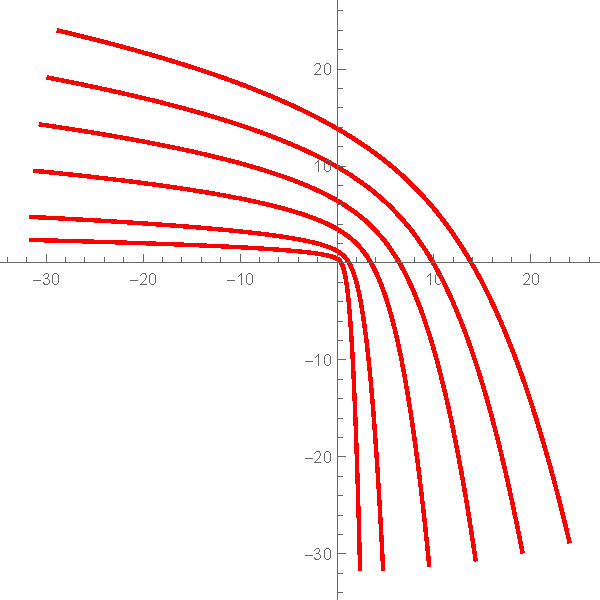
\includegraphics[width=0.6\linewidth]{contour2.pdf}
	\caption{Streamlines around corner}
	\label{fig:4}
\end{figure}
%%%%%%%%%%%%%%%%%%%%%%%%%%%%%%%%%%%%%%%%%%%%%%%%%%%%%%%%%%%%%%%%%%%%
%%%%%%%%%%%%%%%%%%%%%%%%%%%%%%%%%%%%%%%%%%%%%%%%%%%%%%%%%%%%%%%%%%%%
\newpage
\section*{Homework 3\\\\
	Taro V. Brown}\vspace*{1cm}
\section*{Problem 1}
\subsection*{Integral 1}
We want to calulate the integral
\begin{equation}
I_1=\int_{0}^{\infty}\dd x\frac{x^{-a}}{x+1},~~~~~\alpha \in (0,1)
\end{equation}
If we extend this to the complex plane we need to specify a contour which avoids the branch cut along the real axis. A suitable contour is the keyhole (Pacman) contour, see figure
\begin{figure}[H]
	\centering
	\begin{tikzpicture}
		% Configurable parameters
		\def\gap{0.3}
		\def\bigradius{3}
		\def\littleradius{0.5}
		
		% Axes
		\draw (-1.1*\bigradius, 0) -- (1.1*\bigradius,0) node[right] {$\Re$}
		(0, -1.1*\bigradius) -- (0, 1.1*\bigradius) node[above] {$\Im$};
		% Red path
		\draw[red, thick,   decoration={ markings,
			mark=at position 0.17 with {\arrow{latex}}, 
			mark=at position 0.53 with {\arrow{latex}},
			mark=at position 0.755 with {\arrow{latex}},  
			mark=at position 0.955 with {\arrow{latex}}}, 
		postaction={decorate}]  
		let
		\n1 = {asin(\gap/2/\bigradius)},
		\n2 = {asin(\gap/2/\littleradius)}
		in (\n1:\bigradius) arc (\n1:360-\n1:\bigradius)
		-- (-\n2:\littleradius) arc (-\n2:-360+\n2:\littleradius)
		-- cycle;
		\draw [thick,decorate, decoration=zigzag] (0, 0) -- (3, 0);
		\node at (1.5,0.5) {$C_U$};
		\node at (1.5,-0.5) {$C_L$};
		\node at (-0.5,0.7) {$C_\epsilon$};
		\node at (2,2.7) {$C_R$};
	\end{tikzpicture}
\end{figure}
We then have the contour integral
\begin{equation}
\oint_C\dd z\frac{z^{-a}}{z+1},~~~~~\alpha \in (0,1)
\end{equation}
We start of by noting that the large and small circle contours don't contribute since, by parameterizing and assuming there is no residue at $z=0$\footnote{equivalently we can effectively ignore the $\epsilon$ factor in the denominator} we obtain the integrands integrated from $0$ to $2\pi$
\begin{equation}
\begin{aligned}
	iRe^{i\theta}\dd z\frac{e^{-i\alpha\theta }R^{-a}}{e^{i\theta }R+1}\sim R^{-\alpha}\to 0~~~~\text{ as }~~R\to\infty,~~~~~\text{for }\alpha \in (0,1)\\
	i\epsilon e^{i\theta}\dd z\frac{e^{-i\alpha\theta }\epsilon^{-a}}{e^{i\theta }\epsilon+1}\sim \epsilon^{1-\alpha}\to 0~~~~\text{ as }~~\epsilon\to0,~~~~~\text{for }\alpha \in (0,1)
\end{aligned}
\end{equation}
on the upper contour $z=xe^{0i}$ and on the lower $z=xe^{2\pi i}$, with the only pole inseide the contour being the simple pole at $z=-1=e^{i\pi}$. The residue on this pole is easily seen to be $(-1)^{\alpha}=e^{-i\pi \alpha}$ and so the residue theorem then gives (after flipping the integration ranges one of the contours)
\begin{equation}
\begin{aligned}
2\pi i e^{-i\pi \alpha}&=\int_{0}^{\infty}\dd x\,\frac{x^{-\alpha}}{1+x}-\int_{0}^{\infty}\dd x\,\frac{x^{-\alpha}e^{-2\pi i\alpha}}{1+xe^{-2\pi i}}\\
&=\left(1-e^{-2\pi i \alpha}\right)\int_{0}^{\infty}\dd x\,\frac{x^{-\alpha}}{1+x}
\end{aligned}
\end{equation}
which gives us the value of the integral we were looking for, since
\begin{equation}
	\begin{aligned}
		\int_{0}^{\infty}\dd x\,\frac{x^{-\alpha}}{1+x}&=\frac{2\pi ie^{-i\pi \alpha}}{1- ie^{-2i\pi \alpha}}=\frac{\pi}{\sin \pi\alpha}
	\end{aligned}
	\end{equation}
\subsection*{Integral 2}
We now look at the integral
\begin{equation}
I_2=\int_{0}^{\pi}\dd x\,\log(\sin x)
\end{equation}
For this we consider the complex integral 
\begin{equation}
\oint \dd z\,\log(-2ie^{iz}\sin z)
\end{equation}
along the following dented rectangle contour
% TODO: \usepackage{graphicx} required
\begin{figure}[H]
	\centering
	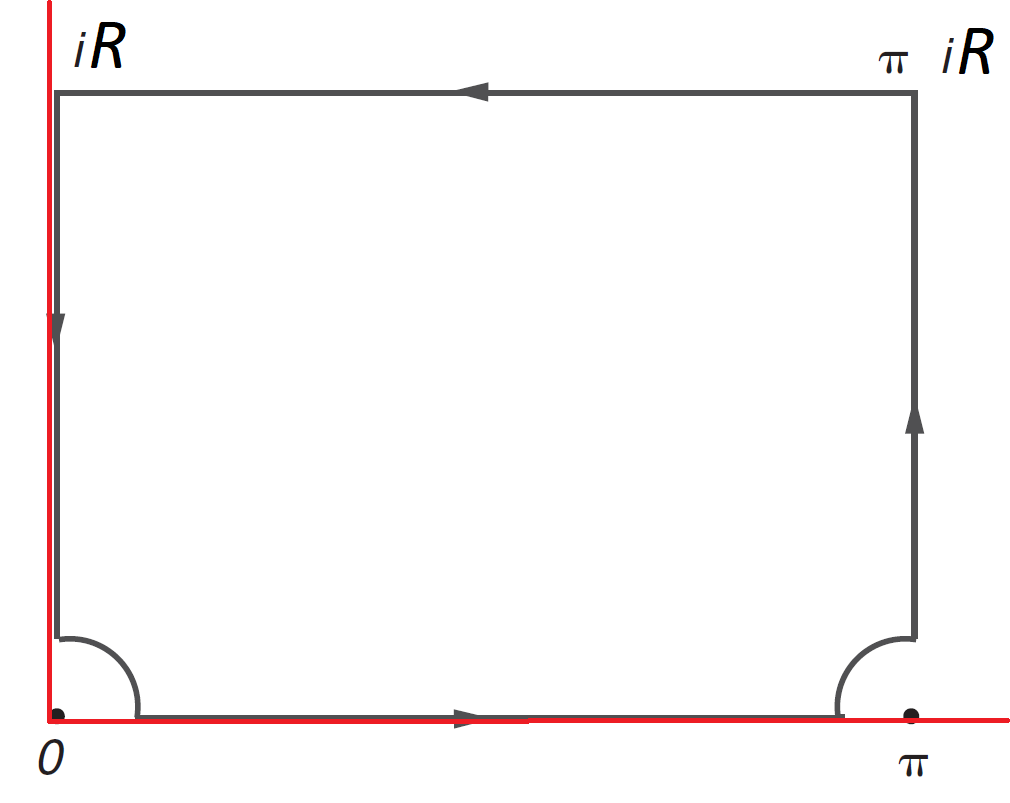
\includegraphics[width=0.5\linewidth]{rectangle}
	\caption{Indented rectangle contour}
	\label{fig:rectangle}
\end{figure}
The integrand is analytic inside this closed contour, and since there are no poles within the contour we get from the residue theorem that the integral along the closed contour vanishes. \\
We start off by looking at the integrand around the indentations. Here we get parameterizations $\epsilon e^{i\theta}$ and $\epsilon e^{i\theta}+\pi$. So the integrands go as
\begin{equation}
\begin{aligned}
&\epsilon \log(-2ie^{i\epsilon e^{i\theta}}\sin {\epsilon e^{i\theta}})\to 0\text{ as } \epsilon \to 0\\
&\epsilon \log(-2ie^{i (\pi +\epsilon e^{i\theta})}\sin {(\pi +\epsilon e^{i\theta})})\to 0\text{ as } \epsilon \to 0
\end{aligned}
\end{equation}
We now find the sum of the integrals of the two vertical contours (parameterizing $z=iR$ in the first and $z=iR+\pi$ on the second)
\begin{equation}
\begin{aligned}
&i\int_{\infty}^{0}\log(-2ie^{-R}\sin iR)+i\int_{0}^{\infty}\log(-2ie^{-R+i\pi}\sin iR+\pi)\\
&=i\int_{\infty}^{0}\log(-2ie^{-R}\sin iR)+i\int_{0}^{\infty}\log(-2ie^{-R}\sin iR)\\
&=
-i\int^{\infty}_{0}\log(-2ie^{-R}\sin iR)+i\int_{0}^{\infty}\log(-2ie^{-R}\sin iR)\\
&=0
\end{aligned}
\end{equation}
For the top of the square we have $z=x+iR$
\begin{equation}
\begin{aligned}
\int_{\pi}^{0}\log(-2ie^{i(x+iR)}\sin (x+iR))
\end{aligned}
\end{equation}
By letting $R\to\infty$ we get that the integrand goes as
\begin{equation}
	\begin{aligned}
\lim_{R\to\infty}\log(-2ie^{i(x+iR)}\sin (x+iR))&=\frac{1}{2} i k e^{i (x+i R)+R-i x}-\frac{1}{2} i k e^{i (x+i R)-R+i x}\\
&=\lim_{R\to\infty} \log(1+e^{2ix-2R})=0
	\end{aligned}
\end{equation}
Finally we see that only the bottom line segment contributes. Here we get
\begin{equation}
	\begin{aligned}
		\int^{\pi}_{0}\log(-2ie^{i(x+iR)}\sin (x+iR))
	\end{aligned}
\end{equation}
\subsection*{Integral 3}
\section*{Problem 2}
\subsection*{Part a}
We want to show that we can use the following integral
\begin{equation}
\begin{aligned}
I_1=\int_0^\infty \dd z\, f(z)\log z
\end{aligned}
\end{equation}
to compute an integral that isn't symmetric and hence can't be computed emidiatly using Jordan's Lemma.
\begin{equation}
	\begin{aligned}
		I=\int_0^\infty \dd x\, f(x)
	\end{aligned}
\end{equation}
Since our integrand now includes the logarithm we must integrate around a contour that excludes the branch cut, see below:
\begin{figure}[H]
	\centering
  \begin{tikzpicture}
	% Configurable parameters
	\def\gap{0.3}
	\def\bigradius{3}
	\def\littleradius{0.5}
	
	% Axes
	\draw (-1.1*\bigradius, 0) -- (1.1*\bigradius,0) node[right] {$\Re$}
	(0, -1.1*\bigradius) -- (0, 1.1*\bigradius) node[above] {$\Im$};
	% Red path
	\draw[red, thick,   decoration={ markings,
		mark=at position 0.17 with {\arrow{latex}}, 
		mark=at position 0.53 with {\arrow{latex}},
		mark=at position 0.755 with {\arrow{latex}},  
		mark=at position 0.955 with {\arrow{latex}}}, 
	postaction={decorate}]  
	let
	\n1 = {asin(\gap/2/\bigradius)},
	\n2 = {asin(\gap/2/\littleradius)}
	in (\n1:\bigradius) arc (\n1:360-\n1:\bigradius)
	-- (-\n2:\littleradius) arc (-\n2:-360+\n2:\littleradius)
	-- cycle;
	\draw [thick,decorate, decoration=zigzag] (0, 0) -- (3, 0);
	\node at (1.5,0.5) {$C_U$};
	\node at (1.5,-0.5) {$C_L$};
	\node at (-0.5,0.7) {$C_\epsilon$};
	\node at (2,2.7) {$C_R$};
\end{tikzpicture}
\end{figure}
The contour segments are
\begin{equation}
\begin{aligned}
C_R:&~~~~~~~~\text{A circle of radius R}\\
C_\epsilon:&~~~~~~~~\text{A circle of radius }\epsilon\\
C_U:&~~~~~~~~\text{Line segment from $\epsilon+i\epsilon$ to $R+i\epsilon$}\\
C_L:&~~~~~~~~\text{Line segment from from $R-i\epsilon$ to $\epsilon-i\epsilon$}
\end{aligned}
\end{equation}
where we take $\epsilon\to 0$ and $R\to \infty$ at the end. This limit should in most cases (but has to be checked) make the contributions from the large and small circles go to zero and so we are left with the discontuniuty over the branch cut. If we look at the two line segments we get two integrals that are restricted along real line (almost)
\begin{equation}
\begin{aligned}
\int_{C_U}\dd z\, f(z)\log z=\int_{\epsilon}^{R} \dd x\, f(x+i \epsilon)\log (x+i\epsilon)\\
\int_{C_L}\dd z\, f(z)\log z=\int_{R}^{\epsilon} \dd x\, f(x-i \epsilon)\log (x-i\epsilon)
\end{aligned}
\end{equation} 
We then use the fact that because of the branch cut
\begin{equation}
\begin{aligned}
\lim_{\epsilon\to 0}\log(x+i\epsilon)&=\log(x)\\
\lim_{\epsilon\to 0}\log(x-i\epsilon)&=\log(x)+2\pi i
\end{aligned}
\end{equation}
Taking the limit we get
\begin{equation}
	\begin{aligned}
		\lim_{\substack{\epsilon\to0\\R\to\infty}}\int_{\epsilon}^{R} \dd x\, f(x+i \epsilon)\log (x+i\epsilon)&=\int^{\infty}_{0} \dd x\, f(x)\log (x)\\
		\lim_{\substack{\epsilon\to0\\R\to\infty}}\int_{R}^{\epsilon} \dd x\, f(x-i \epsilon)\log (x-i\epsilon)&=-\int^{\infty}_{0} \dd x\, f(x)\left(\log (x)+2\pi i\right)\\
	\end{aligned}
\end{equation} 
So that the sum is just
\begin{equation}
\begin{aligned}
\int_{C_U}\dd z\, f(z)\log z+
\int_{C_L}\dd z\, f(z)\log z
&=-2\pi i\int^{\infty}_{0} \dd x\, f(x)\\
&=-2\pi i I
\end{aligned}
\end{equation}
Using this we see that we obtain the integral we wanted provided that the integrals along the large and small circle contours vanish.
In that case we have
\begin{equation}
I=-\sum_{i}\Res[f(z)\log z]_{z=z_i}
\end{equation}
 We can now use this to calculate the following integrals
\begin{equation}
I_a=\int_0^\infty \dd x \frac{1}{(x+1)(x^2+2x+2)},~~~~I_b=\int_0^\infty\dd x \frac{1}{(x^3+1)}
\end{equation}
Performing the firt integral we first check that the contributions from the large and small circles vanish in the appropriate limits by parameterizing $z=Re^{i\theta}$ (large circle) and $z=\epsilon e^{i\theta}$ (small circle). To do this it is convenient to introduce something known as the ML estimate. For an analytic function around some contour $\gamma$ then 
\begin{equation}
\left|\int_\gamma\,\dd z\, f(z)\right|\leq M L
\end{equation}
with L being the length of the contour and M the maximum value of the function on the contour. Taking the large circle contour we parameterize it
\begin{equation}
\begin{aligned}
\int_{C_R} \dd z \frac{\log z}{(x+1)(x^2+2x+2)}&=\int_{0}^{2\pi} i\dd \theta R e^{i\theta} \frac{\log Re^{i\theta}}{(Re^{i\theta}+1)(R^2e^{2i\theta}+2Re^{i\theta}+2)}
\end{aligned}
\end{equation}
The length of the contour is $2\pi R$ and the maximum value is at $2\pi$, so
\begin{equation}
	\begin{aligned}
	 \left|\int_{C_R} \dd z \frac{\log z}{(x+1)(x^2+2x+2)}\right|&\leq(2\pi R)
	 \frac{\log R}{(-R+1)(R^2-2R-2)}\leq2\pi \frac{\log R}{R^2}\to 0 \text{ as } R\to\infty
	\end{aligned}
\end{equation}
For the small circle we will have to assume that the function doesn't blow up around $z=0$. Then the leading order behaviour goes as
\begin{equation}
	\begin{aligned}
		\int_{C_\epsilon} \dd z \frac{\log z}{(x+1)(x^2+2x+2)}&=\int_{\epsilon}^{2\pi-\epsilon} i\dd \theta \epsilon e^{i\theta} \frac{\log \epsilon e^{i\theta}}{(\epsilon e^{i\theta}+1)(\epsilon ^2e^{2i\theta}+2\epsilon e^{i\theta}+2)}\\
			\end{aligned}
	\end{equation}
where the integrand goes as
\begin{equation}
	\begin{aligned}
 \epsilon\log \epsilon \to 0 \text{ as }\epsilon\to 0
	\end{aligned}
\end{equation}
We can now use the residue theorem with the logarithm to find the value of the integral. First factor the integrand
\begin{equation}
\frac{\log z}{(z+1)(z^2+2z+2)}= \frac{\log z}{[z+1]\times \left[z-(i-1)\right]\times \left[z-(-i-1)\right]}
\end{equation}
So we have poles at $\{-1,i-1,-i-1\}$. The exponetial form of these residues are  $\{e^{\pi},\sqrt{2} e^{\frac{3 i \pi }{4}},\sqrt{2} e^{\frac{1}{4} (5 i \pi )}\}$. Taking the residues we then find
\begin{equation}
	\begin{aligned}
	I_a&=-\Res\left[\log z f(z)\right]\Big|_{z=-1}-\Res\left[\log zf(z)\right]\Big|_{z=-1-i}-\Res\left[\log zf(z)\right]\Big|_{z=1-i}\\
	&=-\frac{\log z}{\left[z-(i-1)\right] \left[z-(-i-1)\right]}\Bigg|_{z=-1}-\frac{\log z}{\left[z+1\right] \left[z-(-i-1)\right]}\Bigg|_{z=i-1}-\frac{\log z}{\left[z+1\right] \left[z-(i-1)\right]}\Bigg|_{z=-i-1}\\
	&=-i \pi -\frac{1}{2} \log \left(\frac{1}{2}e^{\frac{5 i \pi }{4}}\right)-\frac{1}{2} \log \left(\frac{1}{2} e^{\frac{3 i \pi }{4}}\right)\\
	&=-i \pi -\frac{1}{2} \log \left(\frac{1}{2}e^{\frac{5 i \pi }{4}}\right)-\frac{1}{2} \log \left(\frac{1}{2} e^{\frac{3 i \pi }{4}}\right)\\
	&=\log 2	\end{aligned}
\end{equation}
For the other integral again use the ML estimate for the large circle contour
\begin{equation}
	\begin{aligned}
		\int_{C_R} \dd z \frac{\log z}{(z^3+1)}&=\int_{0}^{2\pi} i\dd \theta R e^{i\theta} \frac{\log Re^{i\theta}}{(R^3e^{3i\theta}+1)}
	\end{aligned}
\end{equation}
So
\begin{equation}
	\begin{aligned}
		\left|\int_{C_R} \dd z \frac{\log z}{(z^3+1)}\right|&\leq(2\pi R)
		\frac{\log R}{(R^3+1)}\leq2\pi \frac{\log R}{R^2}\to 0 \text{ as } R\to\infty
	\end{aligned}
\end{equation}
While, for the small circle
\begin{equation}
	\begin{aligned}
		\int_{C_\epsilon} \dd z \frac{\log z}{(x+1)(x^2+2x+2)}&=\int_{\epsilon}^{2\pi-\epsilon} i\dd \theta \epsilon e^{i\theta} \frac{\log \epsilon e^{i\theta}}{(\epsilon e^{i\theta}+1)(\epsilon ^2e^{2i\theta}+2\epsilon e^{i\theta}+2)}\\
	\end{aligned}
\end{equation}
where the integrand goes as
\begin{equation}
	\begin{aligned}
		\epsilon\log \epsilon \to 0 \text{ as }\epsilon\to 0
	\end{aligned}
\end{equation}
Hence contributions from both circles vanish. We then factor the integrand like before
\begin{equation}
\begin{aligned}
	\frac{\log z}{(z^3+1)}&= \frac{\log z}{[z-(-1)]\times \left[z-(-1)^{1/3}\right]\times \left[z-(-(-1)^{2/3})\right]}\\
	 &=\frac{\log z}{[z+1)]\times \left[z-(-1)^{1/3}\right]\times \left[z+(-1)^{2/3}\right]}
\end{aligned}
\end{equation}
The residues can also be written as $\{z=e^{i\pi},z=e^{\frac{i \pi }{3}},z=e^{\frac{5 i \pi }{3}}\}$
And evalue the residues at these poles
\begin{equation}\hspace*{-1cm}
	\begin{aligned}
		I_a&=-\Res\left[\log z f(z)\right]\Big|_{z=-1}-\Res\left[\log zf(z)\right]\Big|_{z=(-1)^{1/3}}-\Res\left[\log zf(z)\right]\Big|_{z=-(-1)^{2/3}}\\
		&=-\frac{\log z}{\left[z-(-1)^{1/3}\right] \left[z+(-1)^{2/3}\right]}\Bigg|_{z=-1}-\frac{\log z}{[z+1] \left[z+(-1)^{2/3}\right]}\Bigg|_{z=(-1)^{1/3}}-\frac{\log z}{[z+1] \left[z-(-1)^{1/3}\right]}\Bigg|_{z=-(-1)^{2/3}}\\
		&=-i\pi/3+5/9(-1)^{1/6}+1/9(-1)^{5/6}\pi\\
		&=\frac{2 \pi }{3 \sqrt{3}}
	\end{aligned}
\end{equation}
\subsection*{Problem 3}
\subsection*{Part a}
We want to prove the Mittag-Leffler decomposition
\begin{equation}
f(z)=f(0)+\sum_{j=\infty}^{\infty }r_j\left(\frac{1}{z-z_j}+\frac{1}{z_j}\right)
\end{equation}
First we assume that all the poles of $f(z)$ are simple as well as considering a contour enclosing $n$ poles. Then by the residue theorem we can split this into the poles of $f$ and the pole at $w=z$.
\begin{equation}
\begin{aligned}
\frac{1}{2\pi i}\oint_\gamma \frac{f(w)}{w-z}dw&=\Res(\frac{f(w)}{w-z})\Big|_{w=z}+\sum_j\Res(\frac{f(w)}{w-z})\Big|_{w=z_j}\\
&=\lim_{w\to z}\left(\frac{(w-z)f(w)}{w-z}\right)+\sum_j\lim_{w\to n}\left(\frac{(w-z_j)f(w)}{w-z}\right)\\
&=f(z)+\sum_j\lim_{w\to z_j}\left[\frac{(w-z_j)f(w)}{w-z}\right]\\
\end{aligned}
\end{equation}
The limit on the rhs can be written as a product of the residues of $f$ at $n$ divided by $z_j-z$. Denoting the residues by $r_j$, we then have
\begin{equation}
\begin{aligned}
\frac{1}{2\pi i}\oint_\gamma \frac{f(w)}{w-z}dw&=f(z)+\sum_j\frac{r_j}{z_j-z}\\
\end{aligned}
\end{equation}
Setting $z=0$ we get
\begin{equation}
	\begin{aligned}
		\frac{1}{2\pi i}\oint_\gamma \frac{f(w)}{w}dw&=f(0)+\sum_j\frac{r_j}{z_j}\\
	\end{aligned}
\end{equation}
So we get
\begin{equation}
\frac{1}{2\pi i}\oint_\gamma f(w)\left(\frac{1}{w-z}-\frac{1}{w}\dd w\right)=f(z)-f(0)+\sum_{j=\infty}^{\infty }r_j\left(\frac{1}{z-z_j}+\frac{1}{z_j}\right)
\end{equation}
If we now assume $f(z)$ to be bounded within the contour for all poles then we get the expression requested
\begin{equation}
f(z)=f(0)+\sum_{j=\infty}^{\infty }r_j\left(\frac{1}{z-z_j}+\frac{1}{z_j}\right)
\end{equation}
\subsection*{Part b}
If we assume the function $g(z)$ only has simple poles at positions $z_i$, then the function
\begin{equation}
f(z)=\dv{\log(g(z))}{z}=\frac{g'(z)}{g(z)}
\end{equation}
is meromorphic with the same poles. Residues of these poles can be found using L'Hôpitals rule
\begin{equation}
	\begin{aligned}
\Res(f(z))\big|_{z=z_i}&=\lim_{z\to z_i}(z-z_i)f(z)\\
&=\lim_{z\to z_i}\frac{zg'(z)-z_ig'(z)}{g(z)}\\
&=\lim_{z\to z_i}\frac{g'(z)+zg''(z)-z_ig''(z)}{g'(z)}\\
&=\frac{g'(z_i)}{g'(z_i)}\\
&=1~~~\forall \,i \text{ inside $\gamma$ }
	\end{aligned}
\end{equation}

So 
\begin{equation}
\dv{\log(g(z))}{z}=\frac{g'(z)}{g(z)}\Big|_{z=0}+\sum_{j=-\infty}^{\infty }\left(\frac{1}{z-z_j}+\frac{1}{z_j}\right)
\end{equation}
Integrating up on both sides, we get
\begin{equation}
\log 
\end{equation}
\section*{Problem 4}
\subsection*{Part a}
We consider the function
\begin{equation}
\cot z=\frac{1}{\tan z}
\end{equation}
This has zeroes at $\pi n$ with $n\in \mathds {Z}$. The residues evaluate to $1$ since from L'Hôpitals rule
\begin{equation}
\begin{aligned}
\Res\left[\cot z\right]\Big|_{z=\pi n}&=\lim_{z\to\pi n}(z-\pi n)\cot( z)\\
&=\lim_{z\to\pi n}(z-\pi n)\frac{\cos z}{\sin z}\\
&=\lim_{z\to\pi n}\frac{\cos z-(z-\pi n)\sin z}{\cos z}\\
&=1
\end{aligned}
\end{equation}
Inserting this into the ML expansion, we first subtract the pole at $z=0$
\begin{equation}
\begin{aligned}
\cot z-\frac{1}{z}=\sum_{j=\infty}^{~~\infty ~~,}\left(\frac{1}{z-\pi n}+\frac{1}{\pi n}\right)
\end{aligned}
\end{equation}
The negative and postive parts of the sum converge independently and so we can split the sum as follows
\begin{equation}
	\begin{aligned}
		\cot z-\frac{1}{z}
				&=\sum_{j=1}^{\infty}\left(\frac{1}{z-\pi n}+\frac{1}{\pi n}+\frac{1}{z+\pi n}-\frac{1}{\pi n}\right)\\
		&=\sum_{j=1}^{\infty}\left(\frac{1}{z-\pi n}+\frac{1}{z+\pi n}\right)\\
		&=\sum_{j=1}^{\infty}\left(\frac{2z}{z^2-\pi^2 n^2}\right)
	\end{aligned}
\end{equation}
From this we get the requested equation
\begin{equation} 
	\cot(z)=\frac{1}{z}+\sum_{n=1}^{\infty}\frac{2z}{z^2-\pi^2 n^2}
\end{equation}
Which can also be written in the convention form
\begin{equation} \label{eq:expansion}
	\cot(z\pi)\pi=\frac{1}{z}+\sum_{n=1}^{\infty}\frac{2z}{z^2-n^2}
\end{equation}
%%%%%%%%%%%%%%%%%%%%%%%%%%%%%%%%%%%%%%%%%%%%%%%%%%%%%%%%%
To show the Lipshitz formula we first write the lhs in terms of exponential functions and use the binomial expansion assuming $\Im z>0$
\begin{equation}
	\cot(z\pi)\pi=-\pi i\frac{e^{2\pi iz}+1}{1-e^{2\pi iz}}=-\pi i\left(e^{2\pi iz}+1\right)\sum_{n=0}^{\infty}e^{2n\pi iz}=-2\pi i\left(\frac{1}{2}+\sum_{n=1}^{\infty}e^{2n\pi iz}\right)
\end{equation}
Taking the derivative of this $k\geq 1$ times we obtain
\begin{equation} \label{eq:dcot}
	\dv[k]{\cot(z\pi)\pi}{z}=(-2\pi i)(2\pi i)^{k}\sum_{n=1}^{\infty}n^k e^{2n\pi iz}
\end{equation}
The rhs of \eqref{eq:expansion} can be rewritten by expanding and grouping the sum
\begin{equation}
\frac{1}{z}+\sum_{n=1}^{\infty}\frac{2z}{z^2-n^2}=\frac{1}{z}+\sum_{n=1}^{\infty}\,\left(\frac{1}{z+n}+\frac{1}{z-n}\right)=\lim_{N\to\infty}\sum_{n=-N}^{N}\frac{1}{z+n}
\end{equation}
Now taking the derivative of this $k\geq 1$ times we, while taking the $N\to \infty $ limit, get
\begin{equation}
\sum_{n=-\infty}^{\infty}\frac{1}{(z+n)^k}(-1)^k k!
\end{equation}
Hence combinging this with \eqref{eq:dcot} we get the requested form
\begin{equation}
\sum_{n=-\infty}^{\infty}\frac{1}{(z+n)^k}=\frac{(-2\pi i)^{k+1}}{k!}\sum_{n=1}^{\infty}n^k e^{2\pi iz}
\end{equation}
\subsection*{Part b}
We first note that
\begin{equation}
\cot =
\end{equation}
We first take the ML expansion of $\frac{1}{\sin(z)}$. The residues are at $z=2\pi$ and as before they have value $r_j=1$, so
\begin{equation}
\frac{1}{\sin z}-\frac{1}{z}=\sum_{n=\infty}^{~~\infty ~~,}\left(\frac{1}{z-2\pi n}+\frac{1}{2\pi n}\right)
\end{equation}
\end{document}
